%%%%%%%%%%%%%%%%%%%%%%%%%%%%%%%%%%%%%%%%%%%%%%%%%%%%%%%%%%%%%%%%%
%%% %
%%% % weiiszablon.tex
%%% % The Faculty of Electrical and Computer Engineering
%%% % Rzeszow University Of Technology diploma thesis Template
%%% % Szablon pracy dyplomowej Wydziału Elektrotechniki 
%%% % i Informatyki PRz
%%% % June, 2015
%%%%%%%%%%%%%%%%%%%%%%%%%%%%%%%%%%%%%%%%%%%%%%%%%%%%%%%%%%%%%%%%%

\documentclass[12pt,twoside]{article}
\usepackage[hidelinks]{hyperref}
\usepackage{weiiszablon}
\usepackage{float}
\usepackage{comment}


\author{Beniamin Motyka}

% np. EF-123456, EN-654321, ...
\studentID{EF-160780}

\title{Interaktywny system e-learningowy o zagrożeniach w obszarze cyberbezpieczeństwa}
\titleEN{Interactive e-learning system regarding cybersecurity threats}


%%% wybierz rodzaj pracy wpisując jeden z poniższych numerów: ...
% 1 = inżynierska	% BSc
% 2 = magisterska	% MSc
% 3 = doktorska		% PhD
%%% na miejsce zera w linijce poniżej
\newcommand{\rodzajPracyNo}{1}


%%% promotor
\supervisor{dr Michał Piętal}
%% przykład: dr hab. inż. Józef Nowak, prof. PRz

%%% promotor ze stopniami naukowymi po angielsku
\supervisorEN{dr Michał Piętal}

\abstract{Treść streszczenia po polsku}
\abstractEN{Treść streszczenia po angielsku}

\begin{document}

% strona tytułowa
\maketitle

\blankpage

% spis treści
\tableofcontents

\clearpage
\blankpage

\clearpage
\section*{Wykaz symboli, oznaczeń i skrótów}
\addcontentsline{toc}{section}{Wykaz symboli, oznaczeń i skrótów}

API - (ang. Application Programming Interface) - inferejs programowania aplikacji, zbiór reguł i zasad umożliwiający komunikację pomiędzy aplikacjami, serwisami.

HTML - (ang. Hypertext Markup Language) - język znaczników wykorzystywany do tworzenia dokumentów, które mogą być wyświetlane w przeglądarce internetowej.

CSS - (ang. Cascading Style Sheets) - język arkusza stylów używany do opisywania dokumentu napisanego w języku znaczników, przykładowo HTML.

DOM - (ang. Document Object Model) - interfejs dla plików HTML i XML. Definiuje strukturę dokumentów (np. stron internetowych) w postaci drzewa.

MVC - (ang. Model-View-Controller) - wzorzec projektowy, powszechnie stosowany w procesie tworzenia oprogramowania. 

ORM - (ang. Object–relational mapping) - technika pozwalająca na modyfikację i odczyt danych w relacyjnych bazach danych przy użyciu paradygmatu programowania obiektowego.

SQL - (ang. Structured Query Language) - język stworzony specjalnie w celu komunikowania się z relacyjnymi bazami danych i ich modyfikacji.

XSS - (ang. Cross-site scripting) - jedna z najbardziej niebezpiecznych podatności zagrażająca współczesnym aplikacjom webowym. 

IDS - (ang. Intrusion Detection System) - narzędzia wykrywające próby ataków na systemy teleinformatyczne.

DOS - (ang. Denial-of-Service) - atak na system lub sieć, mający na celu spowodowanie niedostępności serwera lub infrastruktury. Znany również jako Blokada Usług.

UX - (ang. User Experience) - sposób interakcji, doświadczenia użytkownika z systemem.

VR - (ang. Virtual Reality) - sposób wykorzystywania technologii informatycznych celem zasymulowania sytuacji z rzeczywistości.

HTTP - (ang. Hypertext Transfer Protocol) - protokół umożliwiający enkodowanie i przesyłanie informacji pomiędzy klientem (przeglądarką) a serwerem webowym.

REST - (ang. Representational state transfer) - styl architektury oprogramowania standaryzujący sposób komunikacji pomiędzy systemami.

URL - (ang. Uniform Resource Locator) - odniesienie do zasobu internetowego, który określa jego lokalizację w sieci komputerowej.

\clearpage
\section{Wprowadzenie}

W dzisiejszych czasach śmiało można stwierdzić, iż	internet jest istotną częścią codzienności każdego z nas. Ostatnimi laty, stał się on jeszcze bardziej bliskim i niezbędnym narzędziem dla wielu, za sprawą pandemii COVID-19. Sprawiła ona bowiem, że pewne dziedziny życia, takie jak dydaktyka czy praca wykonywana umysłowo, przeszły swoistą transformację. Miejsca, w których spotykali się studenci wraz z wykładowcami, czy pracownicy w biurze, stały się puste. Zastąpiła je komunikacja zdalna -- przez internet. 

Fakt, iż ludzkość została zmuszona, by przenieść znaczną część swojego funkcjonowania do sieci internet, niesie ze sobą poważne konsekwencje. Szybkie jak do tej pory tempo rozwijania się technologii informatycznych stało się nieporównywalnie bardziej dynamiczne, a co się z tym wiąże, obecne w sieci liczne zagrożenia stały się coraz powszechniejsze i trudniejsze w identyfikacji. Pandemia spowodowała również, że znacząco zmienił się profil przeciętnego użytkownika internetu. Poprzez naukę zdalną, uczniowie szkół podstawowych zmuszeni byli do spędzania większej ilości czasu przed ekranami komputerów. Wraz ze zmniejszeniem średniego wieku internauty, zmalała również świadomość dotycząca niebezpieczeństw w sieci, przez co stanowią one większe niż dotychczas zagrożenie. 

\subsection{Cel i zakres pracy}

Celem niniejszej pracy inżynierskiej jest wyeksponowanie, opis oraz implementacja najbardziej pospolitych zagrożeń i luk bezpieczeństwa w internecie nie tylko z perspektywy zwykłych użytkowników, ale również dla małych i średnich przedsiębiorstw (MMŚP). Na podstawie wiedzy wyniesionej ze studiów stworzona została aplikacja internetowa, zwierająca interaktywne kursy o tematyce cyberbezpieczeństwa z elementami wirtualnej rzeczywistości oraz quizami, podsumowującymi wiedzę kursanta po kursie. Każdy kurs składa się ze slajdów, które podzielić można na podstawowe, zawierający zasadnicze informacje na określony temat i zaawansowane, dla kursantów chcących bardziej zgłębić wybrany obszar. Kurs kończy się quizem jednokrotnego wyboru, na którego końcu zostaje przedstawiony wynik zdającego wraz z prawidłowymi odpowiedziami. Ma on na celu zweryfikowanie i ustrukturyzowanie wiedzy użytkownika po ukończonym szkoleniu. Celem zapewnienia większej dostępności szerszemu gronu odbiorców, aplikacja, wraz z treścią kursów, została w całości przetłumaczona na język angielski.

Treść prezentowana podczas kursów wykorzystuje elementy wirtualnej rzeczywistości (VR) w podstawowym stopniu. Kursy pozwalają użytkownikom symulować sytuacje zagrożeń bezpieczeństwa na wirtualnym komputerze czy telefonie. Nie tylko polepsza to końcowe odczucia kursanta, poprzez dostarczenie mu bardziej wartościowej treści, ale także bezpośrednio wpływa na jakość przyswajanej wiedzy. Zostało bowiem udowodnione, że doświadczanie sytuacji zbliżonych do rzeczywistości poprzez interakcję i immersję polepsza proces uczenia się \cite{VrLearning}. 

Dzięki temu, że powyższa idea została zrealizowana w formie aplikacji klasy e-learning wraz z elementami wirtualnej rzeczywistości, istnieje realna szansa na zwiększenie świadomości społecznej, edukację oraz poprawę zabezpieczeń systemów teleinformatycznych i infrastruktury sieciowej. W zakres pracy wlicza się takie zagadnienia jak:
\begin{itemize}
\item Przegląd, dokumentacja i implementacja zagrożeń i luk bezpieczeństwa w sieci. 
\item Przygotowanie i wyselekcjonowanie najważniejszych elementów dla kursantów.
\item Stworzenie aplikacji e-learningowej przy użyciu technologii opisanych w kolejnym rozdziale. Użytkownicy będą mogli wziąć udział w interaktywnej prezentacji każdego z zagrożeń, wraz z weryfikacją efektów kształcenia.
\item Zasugerowanie potencjalnych rozwiązań w odniesieniu do opisanych cyberzagrożeń.
\item Przedstawienie wniosków płynących z powyższych oraz dalszych planów na rozwój projektu.\\
\end{itemize} 

\clearpage

\section{Technologie wykorzystane w aplikacji}

Projekt opisany w niniejszej pracy inżynierskiej składa się z dwóch aplikacji. Pierwsza z nich -- aplikacja działająca po stronie klienta -- została wykonana z użyciem biblioteki React. Jej głównym przeznaczeniem jest warstwa graficzna (UX) z którą użytkownik wchodzi w interakcję. Jest odpowiedzialna za dynamikę strony i wyświetlane na niej treści. Przesyła również informacje od użytkownika do drugiej aplikacji -- API -- która działa stronie serwera i komunikuje się z nierelacyjną bazą danych MongoDB. Opisane API zostało wykonane w technologii GraphQL, w oparciu o środowisko uruchomieniowe Node.js i bibliotekę Express. Architekturę systemu można przedstawić następującym diagramem:

\begin{figure}[H]
	\centering
	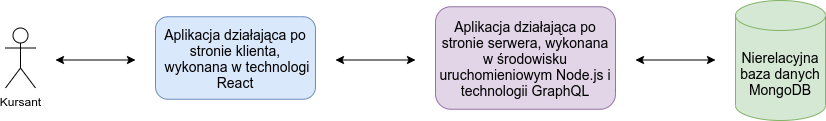
\includegraphics[width=1\linewidth]{figures/app-architecture}
	\caption{Architektura systemu}
	\label{fig:system-architecture}
\end{figure}

\subsection{JavaScript}

JavaScript to skryptowy język programowania powstały w latach 90. ubiegłego wieku, umożliwiający zaimplementowanie na stronach internetowych logiki biznesowej. Dzięki temu strona może nie tylko wyświetlać statyczne treści, ale również wykonywać akcję po wciśnięciu przycisku, kontrolować multimedia, obsługę dynamicznego tworzenia treści... Język ten pozwala również na takie możliwości jak przechowywanie danych wewnątrz zmiennych, wysyłanie żądań do interfejsów programistycznych (API), zarządzanie strukturą drzewa DOM . Dzięki swojemu szerokiemu wachlarzowi zastosowań oraz swoistej elastyczności stał się jednym z podstawowych języków programowania w internecie i od ostatniej dekady znajduje się w pierwszej dziesiątce najpopularniejszych języków programowania. Zgodnie z ankietą przeprowadzoną przez organizację W3Techs, ponad 88\% z około miliarda przeanalizowanych stron internetowych opiera się na tej technologii \cite{JavascriptPopularity}. 

Jest to trzecia warstwa standardowych technologii internetowych, do których należą jeszcze HTML i CSS, łącznie określane jako dHTML (ang. dynamic HTML) \cite{JS}. JavaScript jest obecnie jedynym natywnym językiem programowania dla przeglądarek internetowych, a jego składnia przypomina język C. 

Na bazie tego języka zostało utworzonych wiele szkieletów aplikacyjnych - \emph{frameworków} -  które znacznie przyspieszają i ułatwiają proces budowy aplikacji i interfejsów użytkownika. Do najpopularniejszych z nich należą między innymi React, Vue.js czy AngularJS. Mimo iż wszystkie działają w oparciu o ten sam język, to zazwyczaj kierują się innymi myślami przewodnimi i narzucają różne imperatywy w programowaniu. Dla przykładu - React opiera się o zasady projektowania jak najmniejszych komponentów (cząstek kodu) i łączenia ich w jedną całość, podczas gdy AngularJS działa w oparciu o architekturę MVC.

\subsubsection{React}

React to darmowa biblioteka o otwartych źródłach (ang. open source) stworzona i wspierana przez programistów firmy Facebook. Jej podstawowym celem jest rozdzielenie części interfejsu użytkownika na komponenty -- samodzielne elementy kodu, które mogą być złączone w całość, aby stworzyć pełny widok interfejsu. Oprócz tego zadaniem biblioteki jest zarządzanie stanem treści na stronie i renderowaniem wybranych elementów do drzewa DOM. 

Jednym z kluczowych elementów tej biblioteki jest JSX -- JavaScript XML. Rozszerza to język programowania JavaScript o elementy HTML, dzięki czemu do zmiennych można przypisywać fragmenty kodu HTML:

\

\begin{lstlisting}[language=HTML,caption=Nagłówek strony w wykonany w składni JSX,label={KodJS}]
	const pageHeader = <h2>Header of a page</h2>;
\end{lstlisting}

Zmienne te mogą być odpowiednio renderowane i stylizowane, co zapewnia zorganizowaną i spójną strukturę aplikacji.

Biblioteka ta wprowadza również takie pojęcie jak Wirtualny DOM (ang. Virtual DOM). Jest to replika oryginalnego drzewa DOM przechowywana w wirtualnej pamięci. Przy każdej modyfikacji dowolnego komponentu aplikacji, Wirtualny DOM ponownie renderuje cały interfejs użytkownika. Następnie porównywany jest on z obecnym stanem drzewa i aktualizowane są tylko te komponenty, które zmieniły swój stan. React znajduje sposób na wprowadzenie wszystkich zmian w aplikacji, zachowując przy tym jak najmniejszą liczbę odwołań poprzez interfejs DOM. To sprawia, że jest bardzo wydajny i zoptymalizowany.

Wydawać by się mogło, że omawiana biblioteka, rozszerzając obecne możliwości projektowania interfejsów, może stanowić wyzywanie dla początkujących programistów, ze względu na dość trudną początkową konfigurację projektu oraz zaznajomienie się ze składnią JSX. Jednakże po wykonaniu kilku prostych komponentów, zauważyć można analogię i swoisty standard, który towarzyszy w procesie tworzenia różnorakich elementów interfejsu użytkownika. Za sensem stosowania tej biblioteki przemawiać może badanie firmy Statista, przeprowadzone na programistach aplikacji webowych. React.js zajął w nim pierwsze miejsce, uzyskując popularność w stosowaniu w aplikacjach działających po stronie klienta na poziomie aż 40\% \cite{ReactPopular}.

Oprócz zastosowania w implementacji interfejsów użytkownika dla aplikacji internetowych, biblioteki tej można również używać w celu tworzenia w pełni funkcjonujących aplikacji mobilnych (React Native).

\subsubsection{Node.js}

Z racji rosnącego zainteresowania JavaScript, zaczęto się zastanawiać nad możliwością użycia tego języka programowania poza przeglądarką internetową. W 2008 roku narodziła się idea, dzięki której stworzona została platforma na bazie silnika V8 przeglądarki Google Chrome - Node.js. 

Node.js nie jest serwerem internetowym ani językiem programowania. Jest to wieloplatformowe środowisko uruchomieniowe klasy open source, umożliwiające programistom tworzenie wszelkiego rodzaju narzędzi i aplikacji po stronie serwera w języku JavaScript \cite{NodejsWhatIs}. Aplikacje wykonane w tej technologii mogą być uruchamiane na większości systemów operacyjnych, takich jak Microsoft Windows, Linux, Unix itd.

Środowisko jest przeznaczone do użytku poza przeglądarką -- działa bezpośrednio na systemie operacyjnym urządzenia, pomijając tym samym wszelkie specyficzne dla przeglądarki internetowej API JavaScript, jednocześnie dodając obsługę tradycyjnych interfejsów systemu operacyjnego takich jak biblioteki HTTP czy systemy plików.

Nieodłącznym elementem Node.js jest aplikacja do zarządzania pakietami -- \emph{npm} (ang. node package manager). Jest to jedno z największych na świecie repozytorium oprogramowania, w którym znajduje się ponad 1 300 000 pakietów. Pakietami nazwać można zarówno tzw. frameworki do tworzenia całych aplikacji, takie jak \emph{Express.js} lub \emph{Nest.js}, ale również mniejsze narzędzia, przykładowo \emph{validator}, ułatwiające pracę nad walidowaniem wartości zmiennych.

\emph{Express.js} stworzony został w celu rozszerzenia funkcjonalności środowiska Node.js oraz zaoszczędzenia czasu na powtarzaniu tych samych podstawowych czynności. Ułatwia i automatyzuje skomplikowane operacje związane z systemami API, routingiem, ciasteczkami i nie tylko. Jest powszechnie wykorzystywany w projektach Node.js ze względu na dużą elastyczność (pozwala na przetwarzanie żądań w tzw. warstwie pośredniej), minimalizm i skalowalność.

\subsection{GraphQL}

GraphQL to język zapytań, który udostępnia wspólny interfejs pomiędzy klientem a serwerem do pobierania i zarządzania danymi. Stworzony został w 2012 roku przez inżynierów Facebooka, w 2015 roku zyskał otwarte źródła. Pozwala stronie klienta i serwera na dostęp do danych z wykorzystaniem mniejszej ilości zasobów niż w tradycyjnym REST API. Istotnym jego elementem jest silne typowanie, dzięki któremu definiowane są typy danych wymienialnych pomiędzy klientem a serwerem. GraphQL skupia się bardziej na pobieraniu elementów, podczas gdy REST używany jest do nadania struktury usługom sieciowym. 

W odróżnieniu od API wykonanego w architekturze REST, GraphQL używa tylko jednej metody HTTP do otrzymywania, wysyłania, aktualizowania czy usuwania danych - metody HTTP POST. W tej metodzie, wysyłanej na jeden, wspólny dla wszystkich zapytań adres (zwyczajowo nazywany /graphql) w rdzeniu żądania przesyłane jest 'query expression', czyli wyrażenie zapytania. Tylko i wyłącznie z ciała żądania można wywnioskować, jakiego rodzaju akcja musi zostać podjęta, oraz na jakie zasoby. Zawsze wybierany jest rodzaj operacji, jaka ma być przetworzona. Dwie najczęściej wykonywane operacje to:
\begin{itemize}
	\item query – jest podstawową operacją, znajdującą się praktycznie w każdej aplikacji. Informuje API, że to zapytanie oczekuje jedynie na odpowiedź, nie wprowadza zmian w bazie. W rezultacie zwracane są dane znajdujące się w żądaniu.
	\item mutation – operacja rodzaju \textbf{CUD} (\textbf{C}reate, \textbf{U}pdate, \textbf{D}elete), oczekuje specyficznych danych,
aby wykonać wcześniej zadeklarowaną funkcję.
\end{itemize} 
Zapytania GraphQL nie są w żaden sposób szybsze niż zapytania REST -- cechuje je jednak brak redundancji, gdyż można z nich wybrać konkretne pola, które będą zwrócone. W związku z tym, żądania GraphQL są zawsze mniejsze i bardziej wydajne niż zapytania REST, w których to często zwracane są dodatkowe, niepotrzebne dane.

\subsection{MongoDB}

MongoDB jest nierelacyjną bazą danych zorientowaną na obiekty zwane dokumentami. W przeciwieństwie do baz relacyjnych nie używa ona tabel, rzędów czy kolumn do składowania i odczytu danych. W zamian wykorzystuje kolekcje, w których znajdują się zestawy dokumentów i funkcji, odpowiadające tabelom w relacyjnych bazach danych. Dokumenty składają się z par klucz-wartość. Są to podstawowe jednostki danych. 

Nierelacyjne bazy danych -- w przeciwieństwie do relacyjnych -- cechują się rozszerzalnością horyzontalną, czyli możliwością rozbudowy bazy o dodatkową pamięć masową. Skalowalność wertykalna z kolei skupia się na zwiększeniu mocy obliczeniowej serwera bazy danych, poprzez ulepszenie procesora czy zwiększenie pamięci operacyjnej co generuje znacznie większe koszty, szczególnie przy bazach danych składających się z milionów rekordów. 

Fakt ten sprawia, że bazy NoSQL doskonale wpisują się w trend Big Data (analizy dużych zbiorów danych), ponieważ – w przeciwieństwie do klasycznych silników – pozwalają na szybką analizę niestrukturyzowanych danych i badanie korelacji pomiędzy nimi \cite{BigData}. W tradycyjnej bazie schemat i relacje są w narzucone z góry, a za pomocą odpowiednich zapytań SQL można uzyskać strukturalne odpowiedzi mieszczące się we wcześniej opisanych ramach. W bazie NoSQL nie występuje coś takiego jak schemat - zapewnia to szybszą operację zapisu niż relacyjne bazy, co dodatkowo sprawia, iż nierelacyjne bazy są lepszym wyborem w projektowaniu większych systemów.
 
Baza MongoDB wykorzystywana jest w systemie celem przechowywania treści kursów i artykułów, danych logowania użytkowników, wyników quizów i nie tylko.

\subsection{DeepL}
DeepL to narzędzie stworzone przez firmę DeepL SE. Ten z pozoru zwyczajny translator online tłumaczy teksty za pomocą sztucznych sieci neuronowych. Sieci te trenowane są na milionach przetłumaczonych tekstów, co zapewnia bardzo precyzyjne rezultaty. Trening odbywa się metodą uczenia nadzorowanego -- sieciom pokazywane są różne przykłady tekstów, celem porównania wyników tłumaczenia z tłumaczeniami z danych treningowych. W sytuacji, gdy wystąpią ewentualne rozbieżności, wagi sieci są odpowiednio dostosowywane \cite{Deepl}. Wykorzystanie tej technologi pozwoliło na przetłumaczenie w całości treści strony oraz kursów na język angielski, jednak możliwości tego narzędzia pozwalają również na tłumaczenie tekstów na wiele innych języków. 
 
\clearpage
\section{Zagrożenia bezpieczeństwa}

Zagrożenia opisywane w poniższych podrozdziałach są jednymi z najbardziej niebezpiecznych nie tylko z perspektywy zwykłych użytkowników (phishing, keylogger, ransomware), ale także dla małych i średnich przedsiębiorstw (MMŚP). Warto jednak mieć na uwadze, że opisywane zagrożenia stanowią jedynie małą część wszystkich niebezpieczeństw w sieci.

Każde z opisanych w niniejszej pracy zagrożeń jest rozszerzone w postaci interaktywnego kursu w aplikacji internetowej. W skład kursu wchodzą slajdy, które dzielą się na zaawansowane -- dla użytkowników chcących bardziej zgłębić temat -- oraz podstawowe, dostępne dla wszystkich kursantów. 

Slajd może być interaktywny, o czym świadczą wskaźniki w kształcie rombu, znajdujące się w panelu nawigacji, w dolnej części ekranu. Interaktywne slajdy wymagają od użytkownika wykonania określonej akcji, celem kontynuowania kursu. Dla każdego slajdu dostarczony również jest tekst, sytuację przedstawioną na ekranie. Dodatkowym elementem strony, wspomagającym naukę jest panel notatek, który pozwala na zapisywanie najistotniejszych elementów kursu.

\begin{figure}[H]
	\centering
	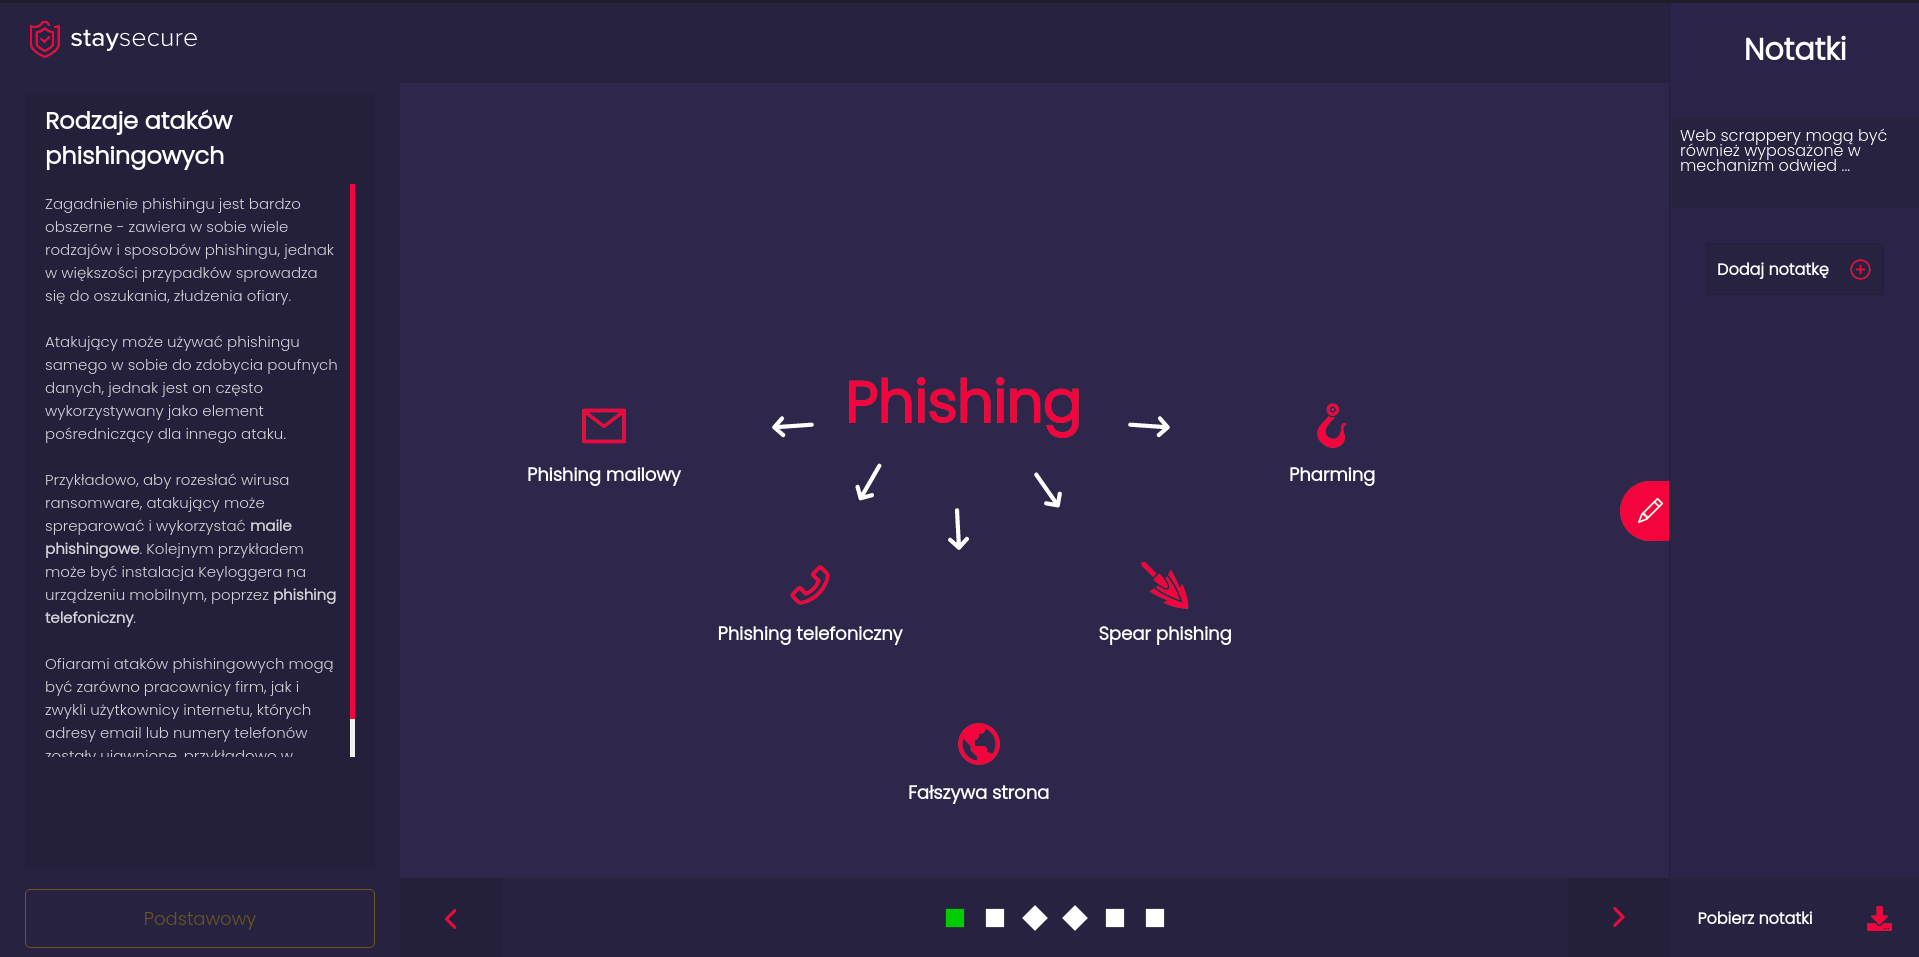
\includegraphics[width=1\linewidth]{figures/slide-tutorial}
	\caption{ sla slajd kursu związanego z tematyką phishingu prezentujący rodzaje ataków phishingowych. Źródło: opracowanie własne}
\end{figure}

\clearpage
\subsection{SQL Injection}

\subsubsection{Opis}

Wstrzyknięcie SQL to podatność aplikacji webowych polegająca na zmodyfikowaniu kwerendy bazodanowej wysyłanej do relacyjnej bazy danych. Celem tego ataku może być uzyskanie informacji, do których w zwyczajnych okolicznościach nie powinno się mieć dostępu: danych personalnych innych użytkowników, ich haseł, numerów kart kredytowych itd. Atak może być wykonany poprzez odpowiednią modyfikację danych wejściowych, np. hasła, produktów w wyszukiwarce, ale także adresu URL (wiedząc, że API działające po stronie serwera wykonane jest w technologii PHP). Podatność może również zostać wykorzystana poprzez zastosowanie serwera proxy, czyli serwera pośredniczącego pomiędzy użytkownikiem a serwerem. Dzięki niemu atakujący może zmodyfikować żądanie wychodzące, tym samym pominąć można wszelką walidację danych wejściowych. 

Ciężko wyobrazić sobie w pełni funkcjonalny serwis internetowy niekorzystający z bazy danych. Proces rejestracji użytkownika, płacenia za zakupy czy zmiana zdjęcia profilowego -- te wszystkie czynności wymagają fizycznego przechowywania informacji. Zazwyczaj realizowane są one poprzez wysłanie odpowiedniego żądania do aplikacji działającej na serwerze, aby ta skomunikowała się z bazą danych i wykonała odpowiednią operację. 

Wykorzystywanie języka SQL w celu podstawowych funkcjonalności może wydawać się proste, ze względu na jego przejrzystość oraz deklaratywną strukturę. Pozwala na łatwe zarządzanie, dostęp do informacji oraz tworzenie i modyfikację struktury bazy danych. Używany jest nie tylko przez programistów w procesie tworzenia API, ale także przez administratorów baz danych, celem dokonywania zmian struktury w schematach bazodanowych.

Najprostsze zapytanie SQL, wypisujące wszystkie dane z tabeli 'clients' można zapisać w poniższej formie:

\

\begin{lstlisting}[language=SQL,caption=Zwrócenie zawartości tabeli 'clients',label={KodSQL1}]
	SELECT * 
	FROM clients
\end{lstlisting}

W zapytaniach bazodanowych może występować również \textbf{selekcja}, która filtruje rekordy wedle danego kryterium. Jest to powszechnie używany zabieg, gdyż zwrócenie jednego konkretnego rekordu, który obecnie jest potrzebny -- przykładowo użytkownika na podstawie jego identyfikatora -- mniej obciąża zasoby instancji bazodanowej i zapobiega wysyłaniu zbędnych informacji poprzez sieć.

\

\begin{lstlisting}[language=SQL,caption=Zwrócenie rekordu o podanym identyfikatorze z tabeli 'clients',label={KodSQL1}]
	SELECT * 
	FROM clients
	WHERE id = "1f168666-432e-401c-bcdc-a70938266a08"
\end{lstlisting}

W wielu sytuacjach, zapytania SQL tworzone są dynamicznie, na podstawie dostarczonych informacji w żądaniu. Przykładowo, użytkownik, wypełniając formularz rejestracji, przesyła do aplikacji 'login' i 'hasło'. Te dane -- jeśli aplikacja jest podatna na atak \emph{SQL Injection} -- są wprost przekazywane do SQL. Poniższe przykłady zapytań aplikacji wykonanej w języku JavaScript prezentują dynamiczne wstawianie wartości, bazując na danych, które mogą pochodzić z formularza nadesłanego przez użytkownika.

\

\begin{lstlisting}[language=SQL,caption=Kod źródłowy zapytania z selekcją na podstawie danych od użytkownika,label={KodSQL2}]
	SELECT * 
	FROM clients
	WHERE login = `${login}` AND password = `${password}`
\end{lstlisting}

\

\begin{lstlisting}[language=SQL,caption=Zapytanie SQL po wprowadzeniu danych,label={KodSQL3}]
	SELECT * 
	FROM clients
	WHERE login = "jankowalski" AND password = "password123"
\end{lstlisting}

Z racji tego, że dane wejściowe nie są w żaden sposób walidowane po stronie serwera, ani odpowiednio formatowane, użytkownik może w bardzo prosty sposób zmodyfikować zapytanie. Przykładowo, w sytuacji, w której zamiast zwykłego loginu zostanie podany ciąg znaków: 

\begin{verbatim}
	jankowalski" OR 1=1 --
\end{verbatim}

SQL wysłane do bazy będzie miało następującą formę:

\

\begin{lstlisting}[language=SQL,caption=Zapytanie wysyłane do bazy po wprowadzeniu zmodyfikowanych danych,label={KodSQL4}]
	SELECT * 
	FROM clients
	WHERE login = "jankowalski" OR 1=1 -- " AND password = "password123"
\end{lstlisting}

Zapytanie o takiej treści zwróci takie rekordy z tabeli clients, w których login to \emph{jankowalski}, lub 1 jest równe 1 (warunek zawsze prawdziwy). Dalsza część kwerendy zostanie uznana za nieważną, ze względu na poprzedzający znak komentarza: ``-\--''. Jako rezultat, w miejsce informacji o użytkowniku z wybranym loginie, zostaną zwrócone wszystkie dane z tabeli. Jest to najpopularniejszy typ ataku wstrzyknięcia SQL. 

Zmodyfikowane zapytania można rozbudować w ten sposób, aby wyświetlały zawartość innych tabel, lub nawet usuwały wybrane tabele.

Przypadek, w którym parametr \emph{login} równy jest:
\begin{verbatim}
	" UNION SELECT credit_card_number from cards --
\end{verbatim}
Efektem czego będzie wykonanie następującego zapytania SQL:

\

\begin{lstlisting}[language=SQL,caption=Zmodyfikowane zapytanie zwracające wrażliwe dane,label={KodSQL5}]
	SELECT * 
	FROM clients
	WHERE login = "" UNION SELECT credit_card_number from cards --" AND password = "password123"
\end{lstlisting}

Zwrócone informacje z bazy danych będą zawierały takie rekordy, w których pole \emph{login} równe jest ``'' (jest puste), oraz wszystkie pola o nazwie \emph{credit\_card\_number} z tabeli \emph{cards}. Spowoduje to zwrócenie atakującemu poufnych informacji o kartach kredytowych, do których nie powinien mieć dostępu.

Przypadek, w którym parametr \emph{password} równy jest:

\begin{verbatim}
	password123"; DROP TABLE clients;--
\end{verbatim}

\

\begin{lstlisting}[language=SQL,caption=Zmodyfikowane zapytanie usuwające tabelę clients,label={KodSQL6}]
	SELECT * 
	FROM clients
	WHERE login = "jankowalski" AND password = "password123"; DROP TABLE clients;--"
\end{lstlisting}	

Rezultatem zapytania będzie najpierw zwrócenie wszelkich rekordów o określonych polach \emph{login} i \emph{password}, a następnie usunięcie tabeli \emph{clients} ze wszystkimi danymi.

Głównym powodem występowania podatności \emph{SQL Injection} jest zbyt mała uwaga poświęcana tworzeniu kwerend bazodanowych przez zespoły programistyczne, w procesie tworzenia aplikacji działających po stronie serwera. Parametry przekazywanego do zapytania powinny być filtrowane pod kątem występowania specjalnych symboli lub pod względem wystąpienia w parametrze określonych znaków, tj. wyłącznie litery i cyfry.

Przy komunikacji z relacyjną bazą danych, dobrym rozwiązaniem może być stosowanie takich narzędzi jak Konstruktora Zapytań (ang. Query Builder) lub ORM pozwala na uproszczenie komunikacji z bazą danych poprzez mapowanie tabel i relacji do obiektów, oraz eliminację możliwości wystąpienia takich luk bezpieczeństwa jak \emph{SQL Injection}. Jako przykład Konstruktora zapytań można podać Knex.js - biblioteka o otwartych źródłach stworzona dla środowiska uruchomieniowego Node.js. Kwerendy tworzone w konstruktorach nie tylko są bezpieczniejsze niż zapytania SQL - są także uniwersalne dla każdego silnika bazodanowego. Konstrukcja zapytań - używając powyżej opisanego konstruktora - przedstawia się następująco:

\

\begin{lstlisting}[language=SQL,caption=Kwerenda bazodanowa stworzona przy użyciu konstruktora zapytań Knex.js,label={KodSQL7}]	
	knex("clients").where({
		login: "${login}",
		password: "${password}"
	}).select('*')
\end{lstlisting}	

Próba wstrzyknięcia SQL do przekazywanego parametru zakończy się błędem w składni Knex.js, w związku z czym poniższa kwerenda nie zostanie wykonana:

\

\begin{lstlisting}[language=SQL,caption=Próba wykonania wstrzyknięcia SQL na konstruktorze zapytań Knex.js ,label={KodSQL8}]	
	knex("clients").where({
		login: "jankowalski" OR 1=1 -- ",
		password: "${password}"
	}).select('*')
\end{lstlisting}	

\emph{SQL Injection} jest luką bezpieczeństwa, która może stanowić poważne zagrożenie nie tylko dla systemu bazodanowego, ale również dla całego przedsiębiorstwa. Przy braku odpowiedniej walidacji danych wejściowych można doprowadzić do sytuacji, w której to atakujący uzyska dostęp do poufnych informacji, lub nawet usunie część bazy danych. Mimo tego, iż należy do stosunkowo prostych podatności pod kątem wykonania, a jej początki sięgają roku 1998, wciąż stanowi ona jedną z najbardziej pospolitych i niebezpiecznych podatności aplikacji działających po stronie serwera.

\subsubsection{Implementacja}

Kurs o tematyce \emph{SQL Injection} zawiera w sobie podstawowe informacje związane z budową strony internetowej i aplikacji działającej po stronie serwera. Istotną częścią kursu jest interaktywny slajd, w którym użytkownik może przeanalizować kod źródłowy wirtualnej strony internetowej. 

Na bazie przekazanych informacji w poprzednich slajdach oraz w opisie, kursant musi zaznaczyć kursorem myszy funkcję w kodzie źródłowym strony, odpowiadającą za przesłanie zawartości formularza.

\begin{figure}[H]
	\centering
	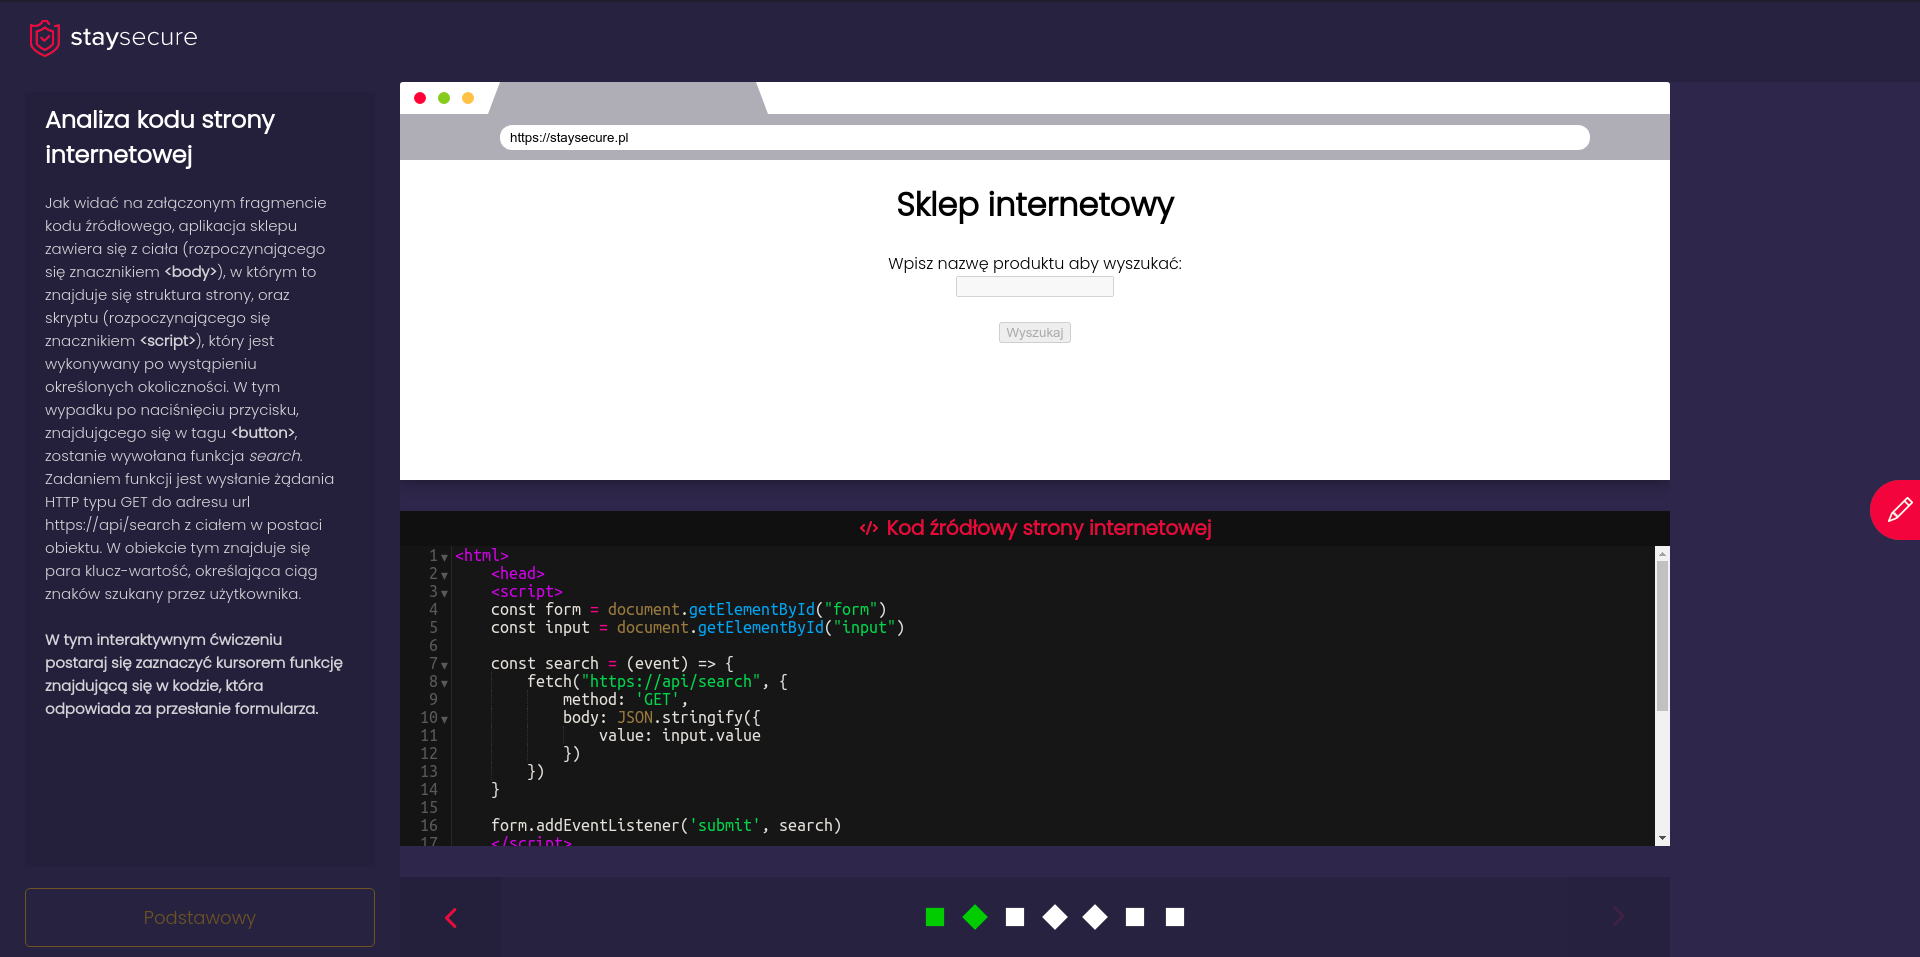
\includegraphics[width=1\linewidth]{figures/sql-slide-screenshot1.png}
	\caption{Interaktywny slajd przedstawiający budowę omawianej strony. Źródło: opracowanie własne}
	\label{Fig:Interaktywny slajd przedstawiający budowę omawianej strony}
\end{figure} 

Użytkownicy o zaawansowanym typie konta mogą zdobyć wiedzę na temat serwerów pośredniczących, które są bardzo często wykorzystywane przy tego typu atakach oraz sposobach komunikacji aplikacji działającej po stronie serwera z bazą danych. 

Dzięki tym informacjom, niedostępnym dla kursantów o zwykłym typie konta, są w stanie poszerzyć wiedzę w temacie przedstawianej podatności, co bezpośrednio przekłada się na efekty kształcenia. Jednocześnie, aby w pełni zrozumieć treść slajdu dla użytkowników o zaawansowanym typie konta, wymagana jest znajomość opisywanych konceptów w stopniu podstawowym.

\begin{figure}[H]
	\centering
	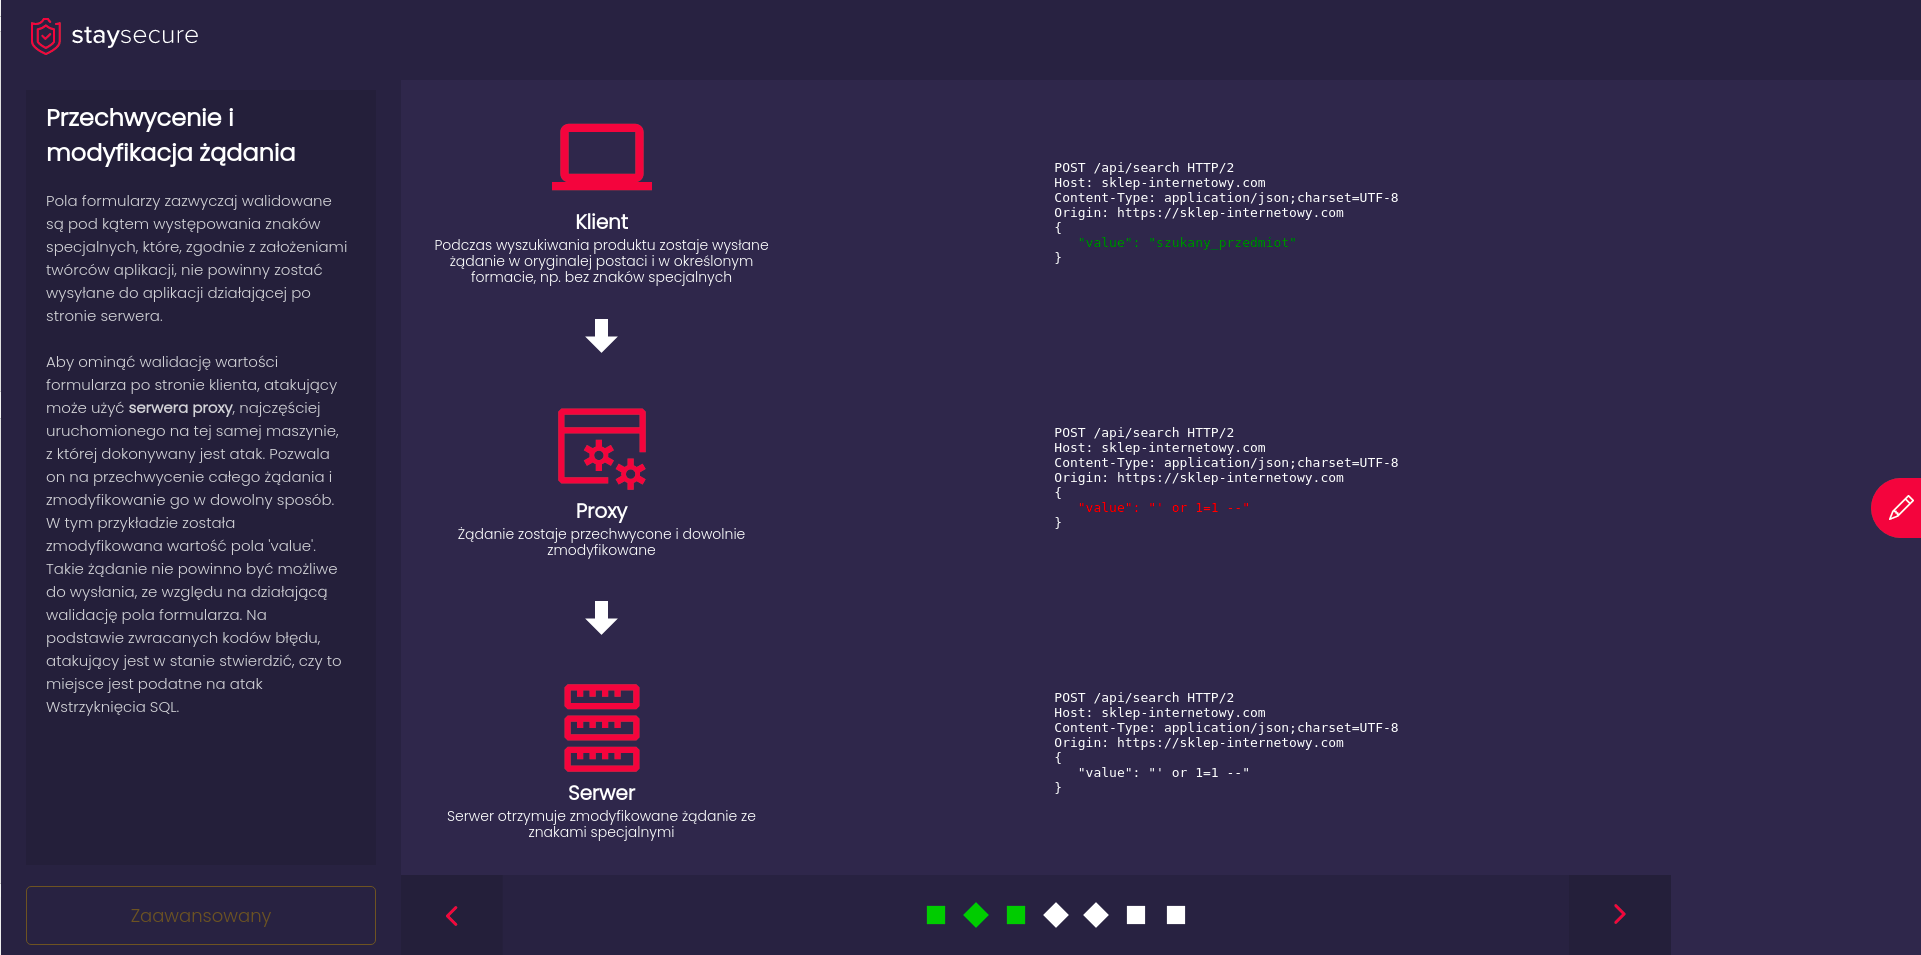
\includegraphics[width=1\linewidth]{figures/sql-slide-screenshot3.png}
	\caption{Slajd przedstawiający działanie serwerów pośredniczących. Źródło: opracowanie własne}
	\label{Fig:Interaktywny slajd przedstawiający budowę omawianej strony}
\end{figure} 

Kluczowym elementem kursu jest analiza kodu aplikacji działającej po stronie serwera, rozpoznanie miejsca, w którym występuje podatność \emph{SQL Injection} oraz próba wykorzystania jej w sytuacji zbliżonej do rzeczywistości. Dzięki możliwie najlepiej odwzorowanemu scenariuszowi, kursant może lepiej zobrazować sposób działania podatności.

Poprzez zastosowanie pakietów typu Open Source z repozytorium \emph{npm}, na stronie zaimplementowany został w pełni działający edytor tekstowy, w którym mógł znaleźć się kod źródłowy aplikacji działającej po stronie serwera oraz strony internetowej. 

Zawarta w interaktywnym slajdzie symulacja, pozwala kursantowi na dowolną manipulację danych wejściowych (formularza na stronie internetowej) i jednocześnie prezentuje, w jaki sposób wartość odczytywana jest po stronie serwera. 

Mając na uwadze informacje przekazane w poprzednich slajdach oraz wskazówki w opisie slajdu, aby kontynuować, kursant musi samodzielnie wykorzystać podatność \emph{SQL Injection} w opisywanym serwisie.

 
 \begin{figure}[H]
 	\centering
 	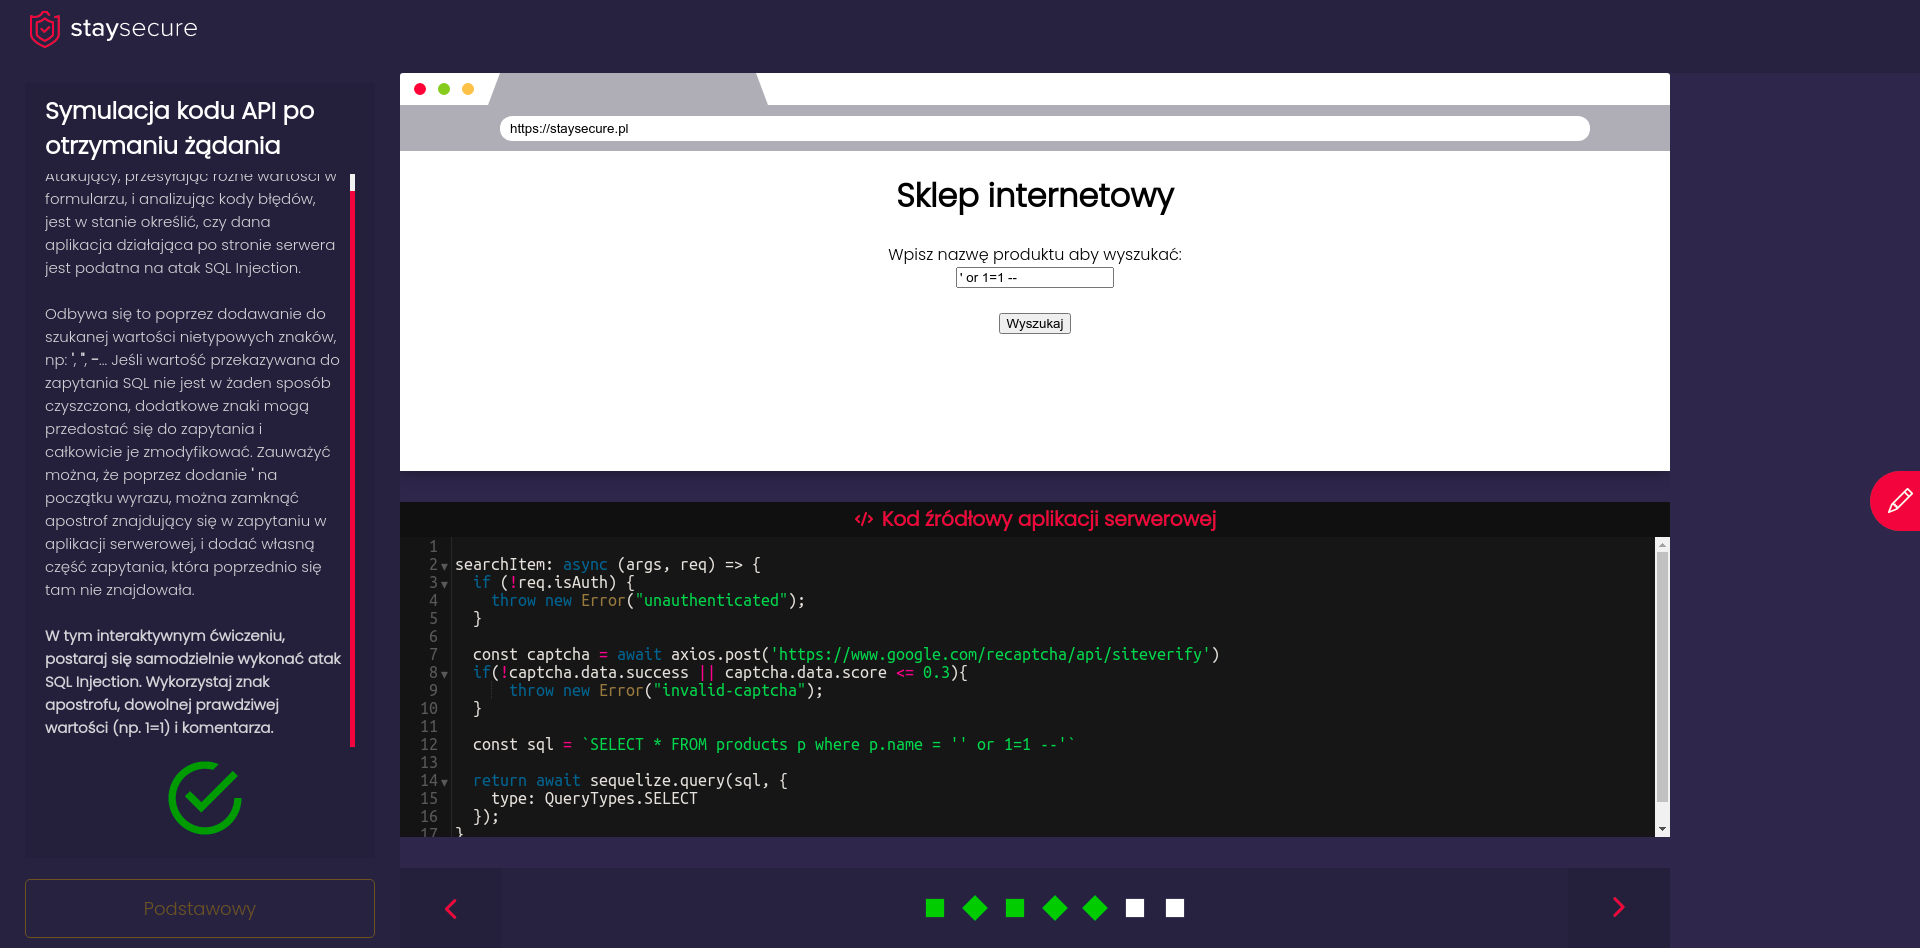
\includegraphics[width=1\linewidth]{figures/sql-slide-screenshot2.png}
 	\caption{Interaktywny slajd przedstawiający kod źródłowy aplikacji działającej po stronie serwera}
 \end{figure} 
 
Opisywany kurs nie wyczerpuje wszystkich przykładów dla zagrożenia \emph{SQL Injection}. Mając na uwadze skomplikowaną naturę tego niebezpieczeństwa i konieczność posiadania podstawowej wiedzy na temat opisywanych zagadnień (bazy danych, język SQL, działanie serwerów webowych) w celu pełnego zrozumienia idei stojącej za tym zagrożeniem, większa ilość informacji mogłaby wydawać się przytłaczająca. 

Ze względu na fakt, iż w kursie zawarte są jedynie kluczowe informacje, jest on łatwiejszy do zrozumienia, a przez to efekt końcowy, w postaci zdobytej wiedzy może być lepszy.

\clearpage

\subsection{Phishing}
\subsubsection{Opis}
Phishing jest pewną formą socjotechniki, w której to atakujący, poprzez podszywanie się pod zaufane osoby lub instytucje, próbuje dokonać nieuczciwego przejęcia poufnych informacji od ofiary. Socjotechnika (inżynieria społeczna) to pewien zestaw sposobów wywierania wpływu na człowieka, aby ten dokonał czegoś wbrew swojej woli. Ataki phishingowe skierowane są zarówno do zwykłych użytkowników, jak i pracowników organizacji rządowych czy korporacji. Organizacja ulegająca atakowi może nie tylko ponieść poważne straty finansowe, ale również stracić reputację i zaufanie konsumentów. Badanie z 2021 r. firmy Kaspersky Lab, tworzącej popularne oprogramowanie antywirusowe Kaspersky wykazuje, że najpopularniejszymi organizacjami wykorzystywanymi przez phisherów są sklepy, portale internetowe i banki.  \cite{PhishingChart}	

\begin{figure}[H]
	\centering
	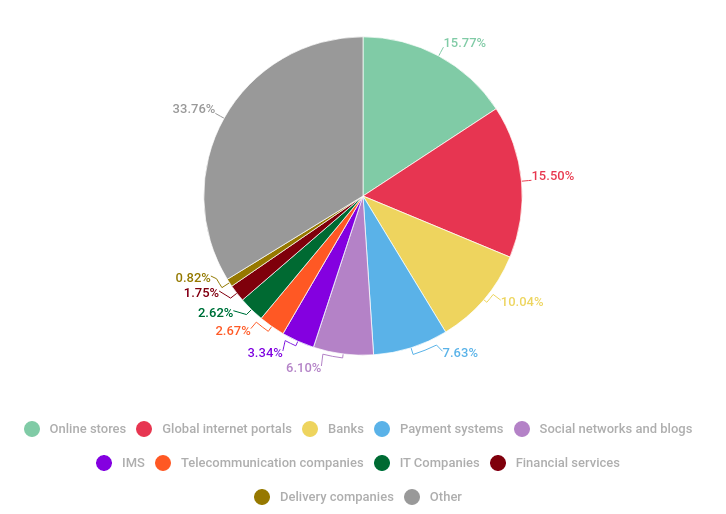
\includegraphics[width=0.9\linewidth]{figures/phishing-organisations}
	\caption{Ranking organizacji wykorzystywanych w atakach phishingowych \cite{PhishingRanking}}
	\label{fig:phishing-organisations}
\end{figure}

Ataki przeprowadzone mogą być używając psychologicznej manipulacji wybranych osób celem uzyskania ich danych osobowych - forma inżynierii społecznej - albo przy użyciu dostępnych narzędzi informatycznych. Najczęściej występujące rodzaje phishingu to:

\begin{itemize}
	\item E-maile phishingowe - spreparowana wiadomość phishingowa wysyłana jest na wiele skrzynek pocztowych, celem zwiększenia prawdopodobieństwa sukcesu ataku. Fałszywe wiadomości mogą zawierać cechy rzekomych organizacji, które miałyby być nadawcami, takie jak logo, stopkę, formatowanie celem skłonienia odbiorców do ujawnienia poufnych informacji, lub wejścia w złośliwe hiperłącze \cite{PhishingEmails}. 
	
	\begin{figure}[H]
		\centering
		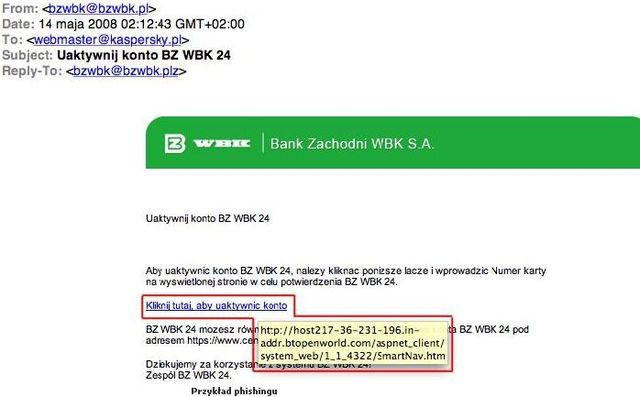
\includegraphics[width=1\linewidth]{figures/phishing-example}
		\caption{Przykład phishingu w formie wiadomości e-mail \cite{PhishingExample}}
		\label{fig:phishing-example}
		
	\end{figure}
	
	\item Fałszywa strona internetowa - polega na stworzeniu zwodniczo podobnej kopii strony internetowej poprzez tzw. \emph{Web Scrapping} \cite{WebScrapping} . Osoba odwiedzająca taką stronę, nie jest w stanie na pierwszy rzut oka odróżnić jej od prawdziwej witryny. Zazwyczaj podstawowe funkcjonalności na sfałszowanym serwisie nie działają, gdyż jego jedynym celem jest przejęcie wrażliwych danych lub kradzież tożsamości użytkownika. Przykładowo, po przesłaniu loginu i hasła, ofiara może zostać przekierowana na zupełnie inną stronę, a dane autoryzacyjne trafią do bazy danych atakującego. Adres strony może być rozpowszechniany poprzez wiadomości phishingowe SMS lub e-mail \cite{WhatIsPhishing}. 
	
	\begin{figure}[H]
		\centering
		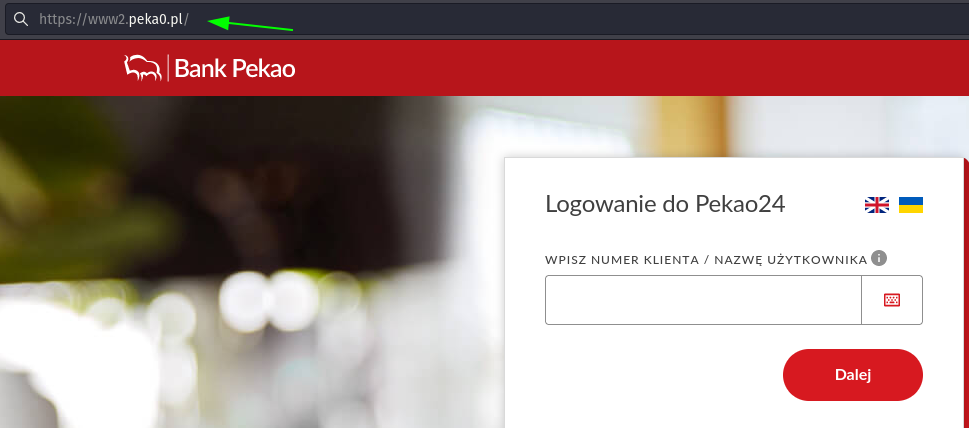
\includegraphics[width=0.96\linewidth]{figures/phishing-example2}
		\caption{Przykład phishingu w formie spreparowanej strony internetowej}
		\label{fig:phishing-example2}
	\end{figure}
	
	\item Phishing telefoniczny - przeprowadzany specyficznie za pomocą wiadomości SMS lub połączeń telefonicznych. Numery telefonów potencjalnych ofiar często pozyskiwane są w wyniku wycieków baz danych przedsiębiorstw lub organizacji. Atakujący kontaktując się z ofiarą, może podawać się za znaną jej osobę lub pracownika zaufanej instytucji, na przykład banku, celem zmanipulowania interlokutora do wykonania określonych akcji.
	\item \emph{Pharming} - rodzaj phishingu, który jest znacznie trudniejszy w detekcji. Polega na zainfekowaniu serwera DNS lub urządzenia użytkownika w ten sposób, aby za każdym razem, gdy odwiedzana jest zaufana strona, nastąpiło przekierowanie na złośliwą, spreparowaną stronę internetową. 
	
\end{itemize}

Wektorami ataków phishingowych w większości przypadków są ludzie, a nie urządzenia. Szczególnie zagrożone są osoby niemające na co dzień styczności z internetem. Dobrym pomysłem jest - tam gdzie to możliwe - stosowanie uwierzytelniania wieloskładnikowego. Polega ono na potwierdzeniu próby autoryzacji poprzez dodatkowy element: kod wysyłany wiadomością SMS lub e-mail. Zapobiega to sytuacjom, w których to dane autoryzacyjne poszkodowanego takie jak adres e-mail i login zostaną użyte przez niewłaściwe osoby. Nie będą one mogły w pełni się uwierzytelnić, jeśli nie posiadają kodu autoryzacyjnego. Dodatkowo może stanowić ostrzeżenie dla ofiary, że ktoś próbuje zalogować się na jej konto. Zaufanym rozwiązaniem są również programy antywirusowe, ostrzegające użytkownika przed fałszywymi domenami oraz odpowiednio skonfigurowane filtry anty-spamowe w poczcie e-mail.

Należy także uważnie sprawdzać adresy URL stron internetowych, na których podaje się wrażliwe dane. Phisherzy często wykorzystują podobieństwo niektórych cyfr i liter, na przykład ``0'' i ``o'' celem stworzenia złudzenia, że użytkownik znajduje się na właściwej stronie. Istotnym elementem jest również protokół, który użyty został do połączenia ze stroną. Zdecydowana większość organizacji korzysta z ważnych certyfikatów SSL, sprawiając, że połączenie między klientem a serwerem jest szyfrowane (HTTPS).

\subsubsection{Implementacja}

Kurs poświęcony tematyce szeroko pojętego phishingu opisuje między innymi typy tego niebezpieczeństwa i metody ochrony przeciw atakom phishingowym. W dzisiejszych czasach, zagrożenie to jest niezwykle powszechne, szczególnie w postaci phishingu SMS, telefonicznego czy stron phishingowych. Właśnie dlatego przedstawione interaktywne slajdy w kursie pozwalają użytkownikowi kontrolować wirtualny smartfon -- urządzenie, które na co dzień używa każdy z nas. 

Kursanci mogą bezpiecznie doświadczyć, jakie mogą być konsekwencje wejścia w podejrzaną stronę internetową w wiadomości SMS.

\begin{figure}[H]
	\centering
	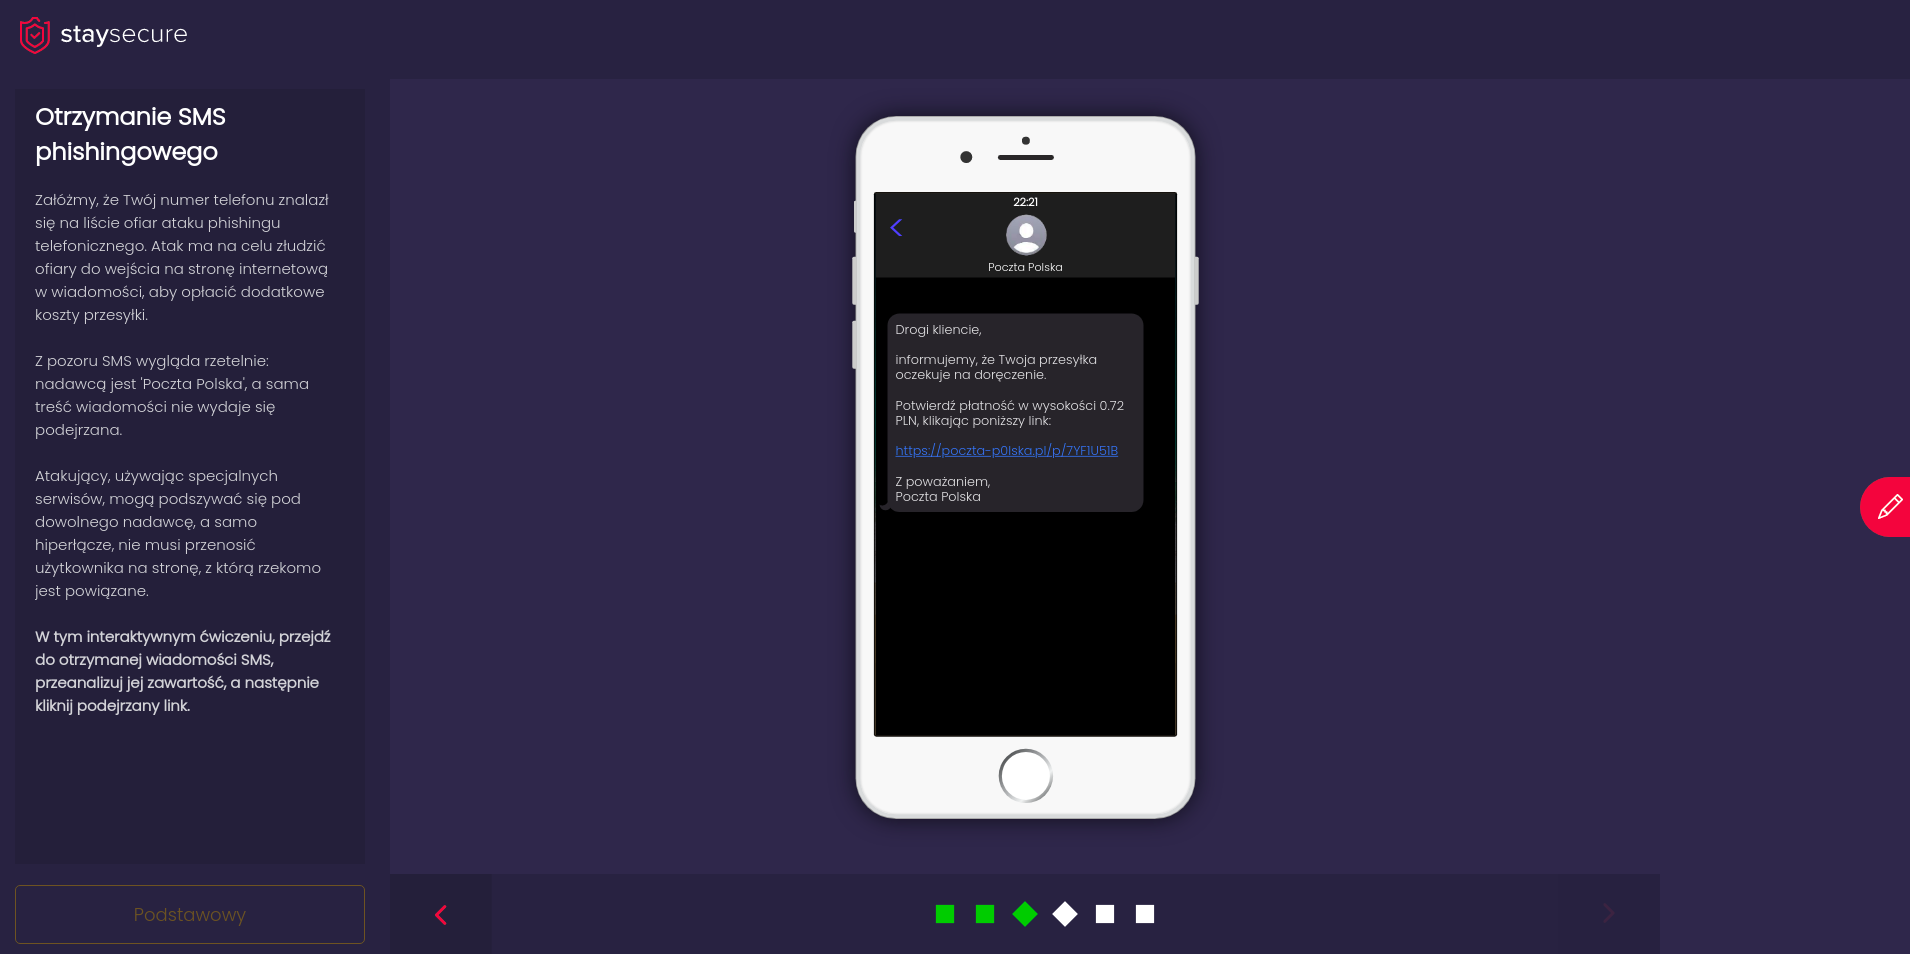
\includegraphics[width=1\linewidth]{figures/phishing-slide-screenshot1.png}
	\caption{Interaktywny slajd przedstawiający otrzymanie phishingowej wiadomości SMS na wirtualnym smartfonie. Źródło: opracowanie własne}
	\label{fig:phishing-organisations}
\end{figure}

Dodatkowo uwypuklone są najistotniejsze elementy ataku, dzięki czemu istnieje realna szansa, że osoba, która ukończy kurs, będzie zwracała większą uwagę i nie padnie ofiarą ataku phishingowego.

\begin{figure}[H]
	\centering
	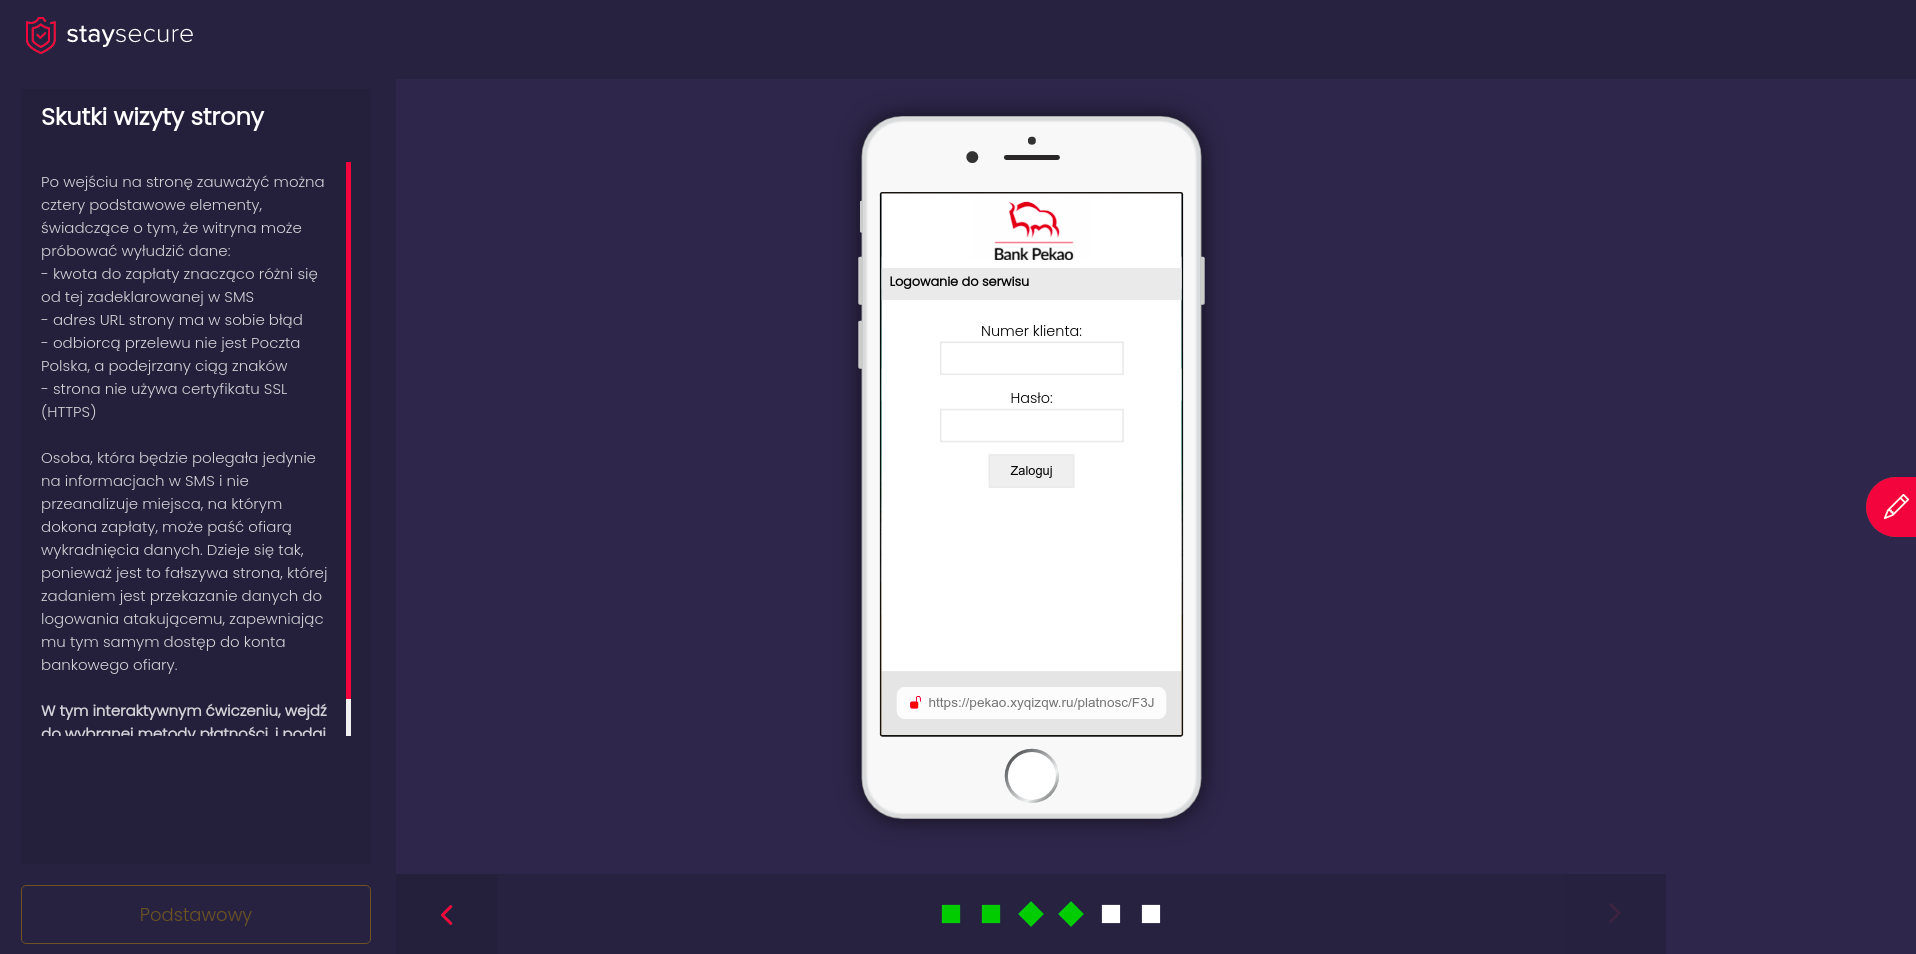
\includegraphics[width=1\linewidth]{figures/phishing-slide-screenshot2.png}
	\caption{Interaktywny slajd przedstawiający stronę phishingwą na wirtualnym smartfonie. Źródło: opracowanie własne}
	\label{fig:phishing-organisations}
\end{figure}

Obszar zagrożeń phishingu jest bardzo szeroki i może obejmować różne typy ataków, jednak w zdecydowanej większości przypadków sprowadza się do wykradnięcia danych ofiary, co jest przedstawione i opisane w treści kursu.

\clearpage

\subsection{Podatność XSS}
\subsubsection{Opis}

XSS jest atakiem skierowanym na klienta korzystającego serwisu webowego, w przeciwieństwie do np. \emph{SQL Injection}, którego celem jest aplikacja działająca po stronie serwera. \emph{Cross-site scripting} opiera się głównie na wstrzyknięciu do strony internetowej złośliwego skryptu, który, dla przykładu, może odczytać ciasteczka użytkownika lub inne poufne informacje, które przechowuje przeglądarka, wysłać je do atakującego, aby ten -- używając zapisanych w ciasteczkach danych -- mógł zalogować się na konto użytkownika, który nieświadomie uruchomił dany skrypt. % Poprzez ten atak, można również uruchomić Keyloggera (narzędzie do przechwytywania aktywności klawiatury) działającego w przeglądarce, lub całkowicie zmienić zawartość strony internetowej. 

W raporcie przygotowanym w 2017 roku przez Wordfence, komercyjną organizację zajmującą się zabezpieczaniem stron internetowych przed wszelkimi niebezpieczeństwami, wynika, iż ten typ podatności stanowi blisko połowę wszystkich podatności w sieci.

\begin{figure}[H]
	\centering
	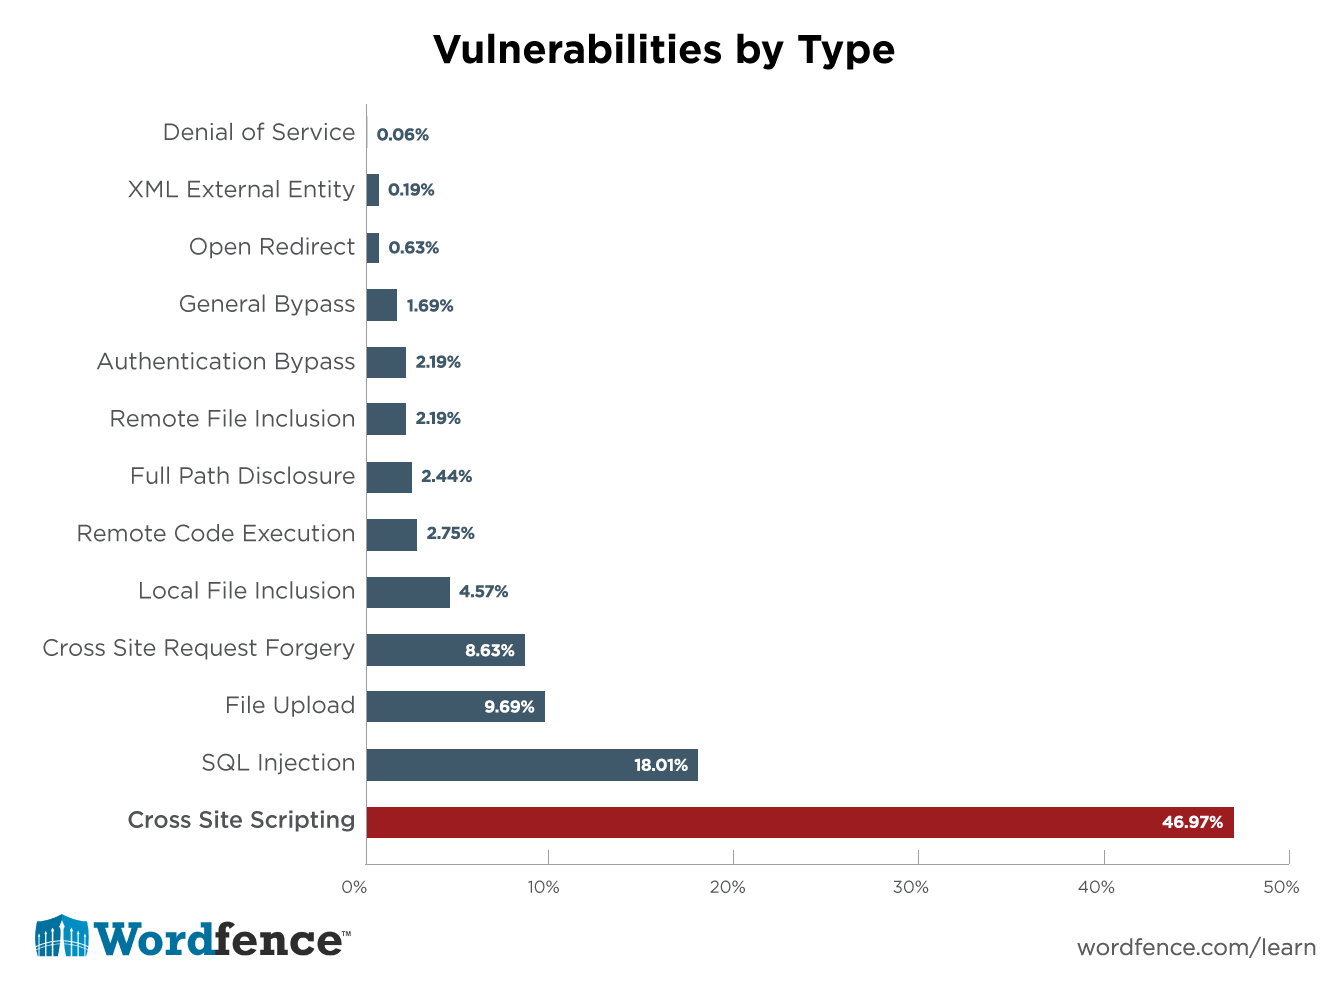
\includegraphics[width=0.9\linewidth]{figures/xss-popularity}
	\caption{Klasyfikacja podatności aplikacji internetowych pod kątem częstotliwości występowania \cite{XSSReport}}
	\label{fig:xss-popularity}
\end{figure}



Opisując XSS nie sposób nie wspomnieć o Regule Tego Samego Pochodzenia (\emph{Same-Origin Policy}) \cite{SameOriginPolicy}. Jest to jeden z wielu fundamentalnych mechanizmów bezpieczeństwa, zaimplementowany w każdej przeglądarce internetowej. Nie pozwala on żadnej stronie na podjęcie akcji lub odczytania zawartości innej strony, na przykład w dwóch kartach przeglądarki. W związku z tym, wszystko, co się dzieje na stronie internetowej otwartej przez użytkownika, jest izolowane i nie będzie miało wpływu na pozostałe otwarte strony. Narzędziami powiązanymi z opisaną polityką są piaskownice (ang. sandbox), pozwalające na uruchamianie programów komputerowych nieznanego pochodzenia w odizolowanym środowisku. Dzięki temu, uruchomienie jakiegokolwiek wirusa bądź wejście w podejrzany link nie zainfekuje urządzenia.
	
	Cała struktura strony internetowej zakodowana językiem HTML może być zmieniana poprzez JavaScript, używając DOM API \cite{DOM}. Jako rezultat, prosty skrypt może całkowicie zmienić zawartość, wygląd, a przede wszystkim funkcjonalność strony internetowej.
	
	Ciasteczkami (ang. cookies) \cite{Cookies} nazywa się niewielkie porcje informacji wysyłane przez serwer do przeglądarki internetowej. Służą do tego, by zapisać obiekty danych w plikach przeglądarki, które przy ponownym odwiedzeniu strony, mogą być przesłane do tego samego serwera, z którego przyszły. W związku z tym, przy odwiedzaniu różnorakich stron wymagających autoryzacji, użytkownik nie musi się za każdym razem logować, gdyż wszystkie potrzebne dane są zawarte w ciasteczkach, które przesyłane są razem z żądaniem. 
	
	Ataki XSS można podzielić na trzy główne kategorie:
	
	\begin{itemize}
		\item \emph{Reflected XSS} - złośliwy skrypt umieszczony jest w adresie URL. Po wejściu w hiperłącze, ofiara nieświadomie wykonuje wcześniej przygotowany skrypt, rezultatem czego jest wykonanie kodu w przeglądarce. Kod umieszczony może zostać w wiadomości e-mail lub w innym serwisie internetowym.
		\item \emph{Stored XSS} - polega na umieszczeniu skryptu po stronie serwera, przykładowo jako wiadomość w serwisie społecznościowym. Po odczytaniu jej przez ofiarę, automatycznie wykonywany jest wcześniej przygotowany skrypt, co może skutkować wysłaniem ciasteczka sesyjnego innego użytkownika do atakującego, pozwalając mu na umieszczenie skradzionego ciasteczka w przeglądarce i nieautoryzowany dostęp do konta ofiary.
		\item \emph{DOM Based XSS} - atak ściśle powiązany z modyfikacją struktury DOM podatnej strony internetowej. Sama odpowiedź HTTP nie ulega zmianie, jednak kod po stronie klienta zawarty w aplikacji wykonywany jest w inny sposób z powodu modyfikacji, które miały miejsce w DOM. Typ ataku szczególnie powszechny w serwisach, które pozwalają użytkownikowi na manipulację zawartości strony, przykładowo poprzez dodanie komentarza. 
	\end{itemize}
	
Przeglądarki internetowe zostały wyposażone wiele narzędzi do walki z tą podatnością, takich system wykrywania złośliwego kodu JavaScript. Mechanizm ten składa się z wbudowanego w przeglądarkę komponentu analizy skryptów oraz systemu IDS, przetwarzającego aktywność po stronie klienta, i porównującego ją ze znanymi złośliwymi skryptami. Dzięki temu systemowi możliwe jest wykrywanie różnego rodzaju ataków XSS. Jednak system ma znaczną wadę: może wykryć tylko sytuacje, których zachowanie jest mu znane -- nie jest odporny na nowe typy ataku \cite{XSSProtection}. 

Najczęstszym miejscem, w którym można spotkać tę podatność, są formularze, do których użytkownik wpisuje dane, które mogą następnie być wyświetlane. Jeśli przesłane dane nie zostaną odpowiednio wyczyszczone, atakujący może wstrzyknąć złośliwy skrypt, który następnie zostanie wykonany przez przeglądarkę. Pomimo wielu zabezpieczeń, które są wbudowane w przeglądarki, te nie są w stanie odróżnić czy dany skrypt jest złośliwy, czy nie - dlatego też odporność aplikacji internetowej na tego typu atak stoi przede wszystkim po stronie programistów.
	
Najskuteczniejszą ochroną przed atakami XSS jest filtrowanie danych przychodzących od użytkownika przed tym, kiedy to mają zostać wyświetlone w aplikacji, na przykład poprzez zamianę znaków tagów HTML na znaki specjalne \cite{XSSSpecialTags}. Skutecznym rozwiązaniem może być także oczyszczanie wprowadzonej treści użytkownika z elementów wspólnych dla każdego ataku XSS, na przykład tagów <script></script>.
	
\subsubsection{Implementacja}

Kurs oprócz opisania cech omawianej podatności pozwala także użytkownikowi na zaznajomienie się z konsekwencjami ataku \emph{Cross-site scripting}. W części interaktywnej kursantowi przedstawiona jest wirtualna strona internetowa podatna na atak \emph{Reflected XSS}, której główną funkcjonalnością jest wyszukanie znajomych. Poprzez efekt immersji, użytkownik jest w stanie łatwiej przyswoić przekazywane mu informacje, gdyż okoliczności mogą wydawać mu się znajome i dotyczą codziennych sytuacji.

\begin{figure}[H]
	\centering
	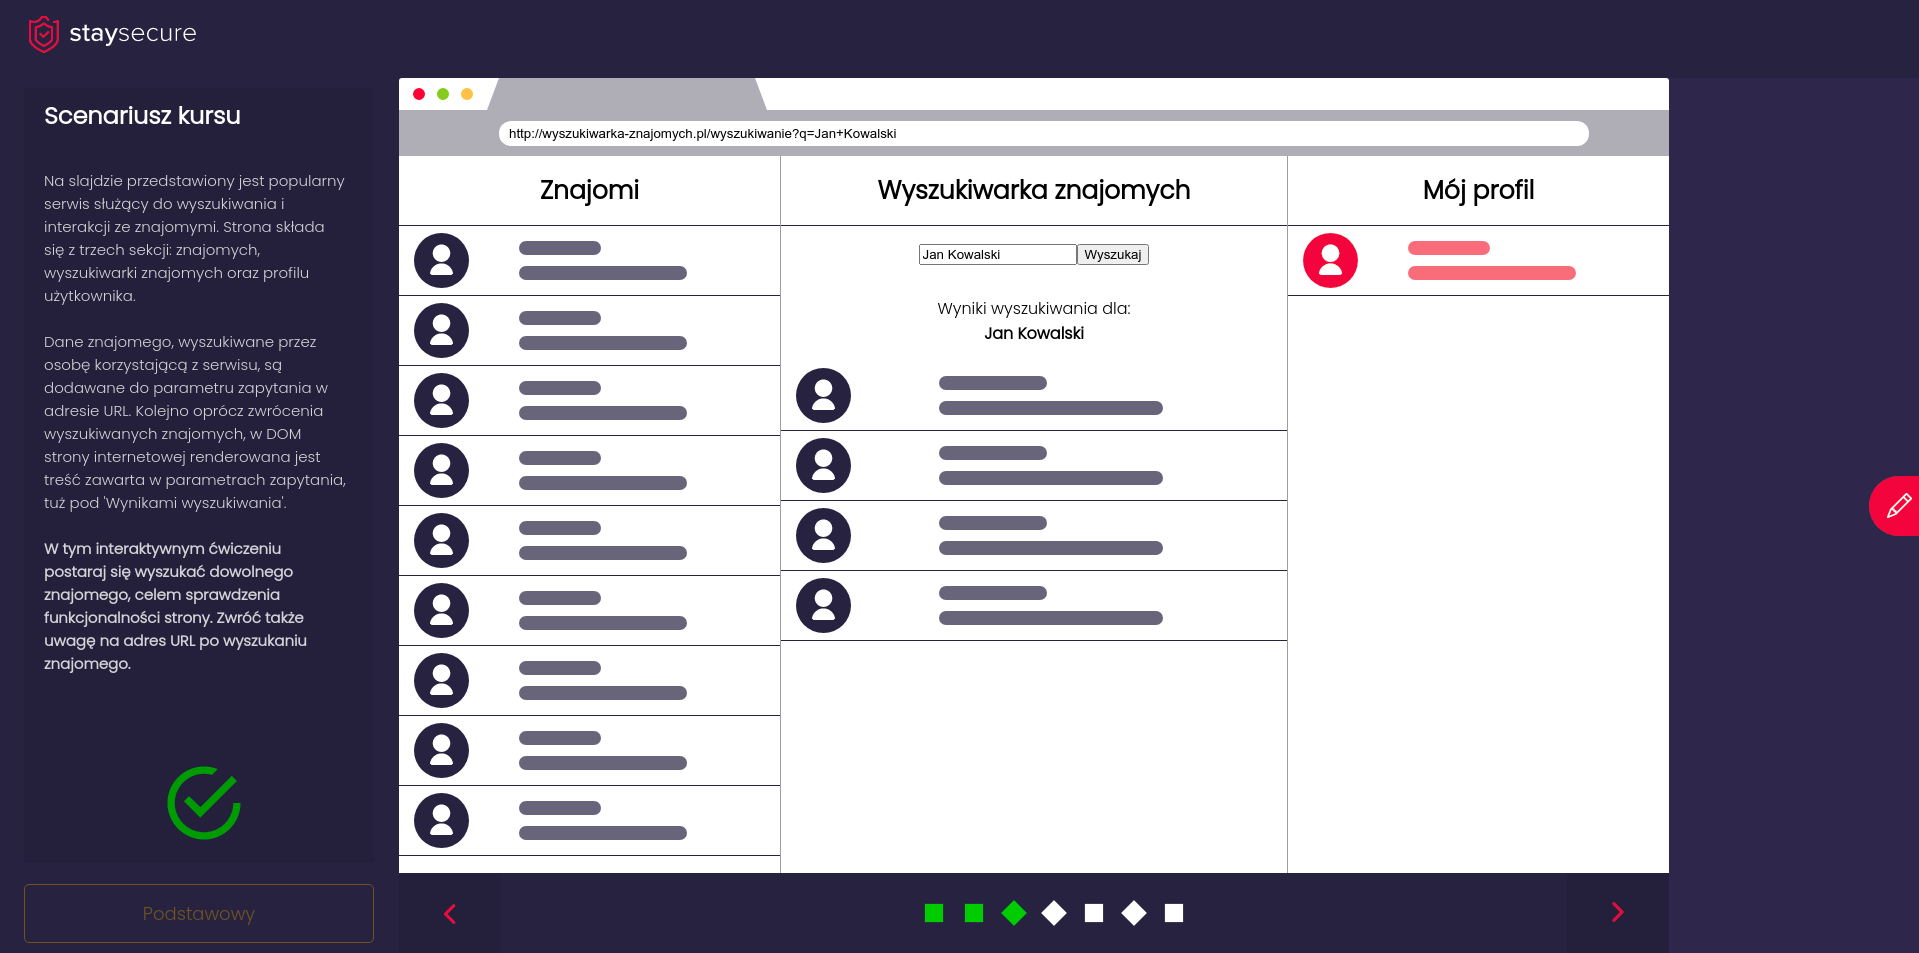
\includegraphics[width=1\linewidth]{figures/xss-slide-screenshot1}
	\caption{Interaktywny slajd przedstawiający podstawowe funkcjonalności wirtualnej strony internetowej. Źródło: opracowanie własne}
\end{figure}

Na bazie informacji zdobytych na wcześniejszych slajdach, w kolejnym interaktywnym ćwiczeniu zadaniem jest wpisanie w pole wyszukiwarki dowolnego elementu HTML. Wyszukanie tagu spowoduje dodanie go do DOM i adresu URL serwisu.

\begin{figure}[H]
	\centering
	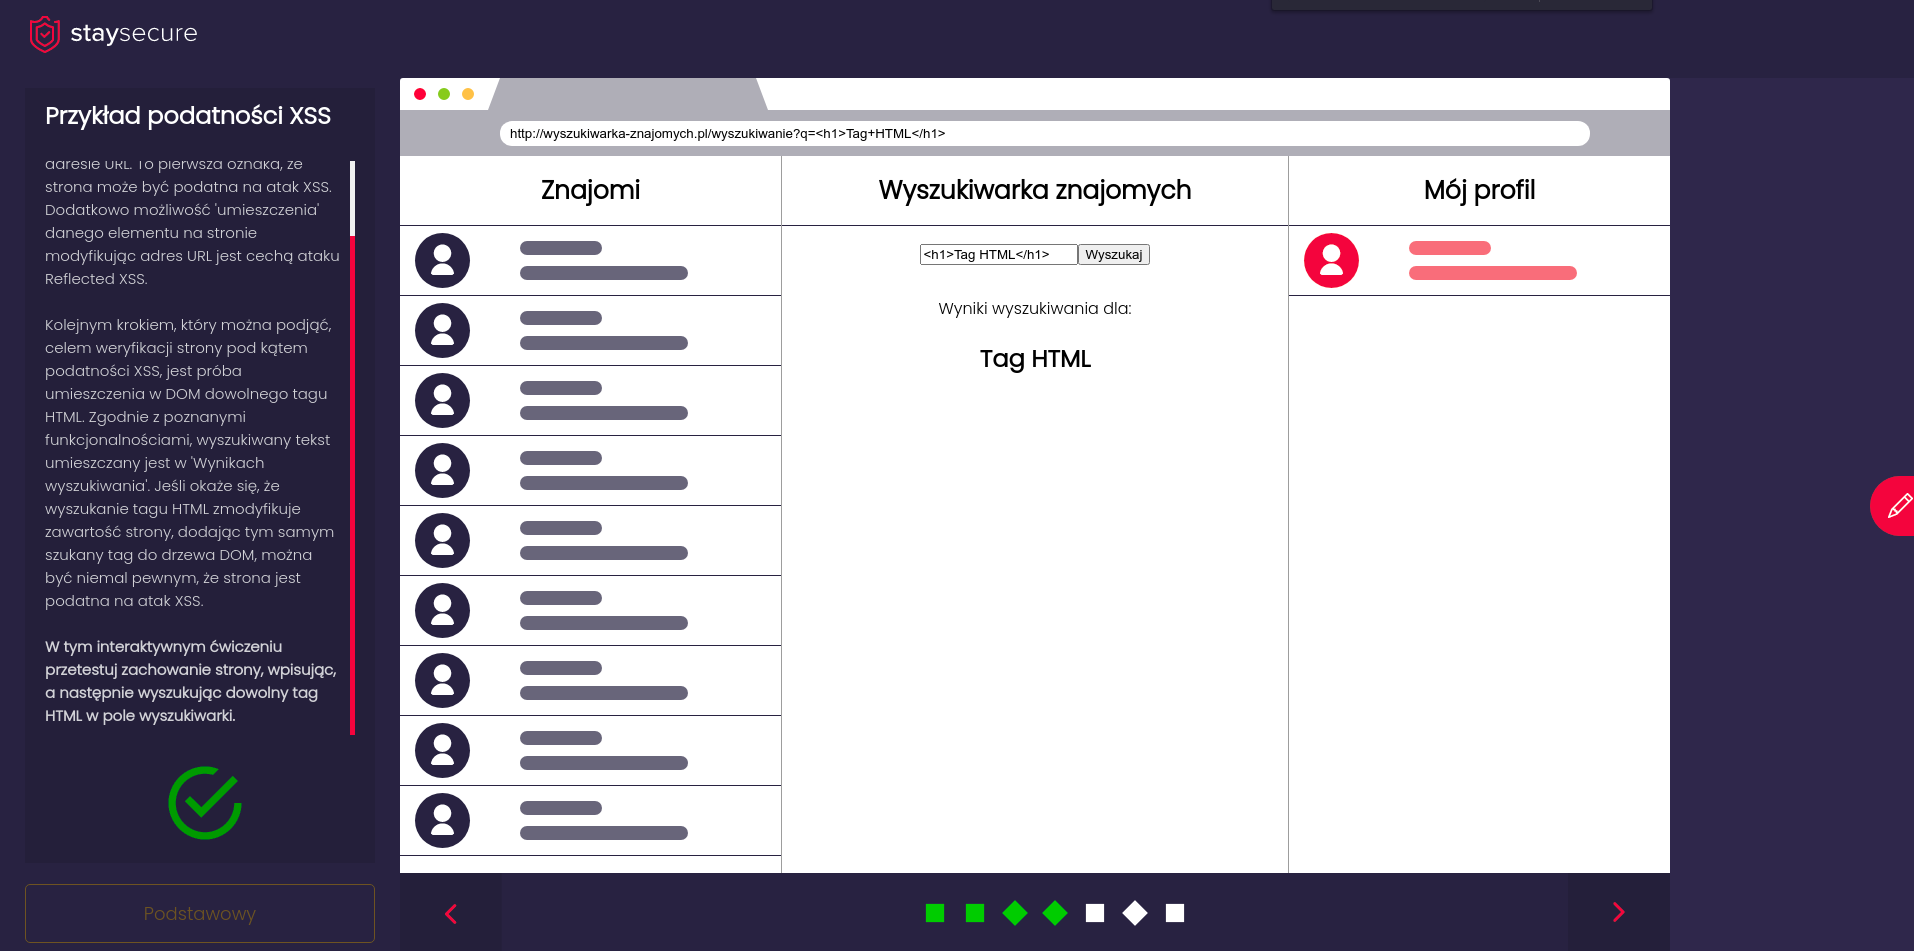
\includegraphics[width=1\linewidth]{figures/xss-slide-screenshot2}
	\caption{Interaktywny slajd przedstawiający podatność XSS. Źródło: opracowanie własne}
\end{figure}

Dzięki zawartości interaktywnych slajdów kursant ma szansę doświadczyć krok po kroku, w jaki sposób wyszukiwana jest opisywana podatność w serwisie internetowym i jakie mogą być jej efekty końcowe. 

Przedstawiony kurs pokrywa tylko jeden typ ataku \emph{Cross-site scripting}. Podobnie jak kurs \emph{SQL Injection}, od użytkownika wymagana jest znajomość technologii składających się na dHTML w stopniu podstawowym. W ramach rozwoju projektu kurs może zostać rozszerzony o przedstawienie innych typów ataku: Stored i DOM Based XSS.


\clearpage

\subsection{Ransomware}
\subsubsection{Opis}
\emph{Ransomware} to typ złośliwego oprogramowania (ang. malware), którego celem jest zablokowanie dostępu do komputera osobistego poprzez zaszyfrowanie wszystkich możliwych plików. Czas trwania tej procedury zależy między innymi od wybranego algorytmu szyfrowania i danych na szyfrowanym urządzeniu, jednak w przypadku zwykłego użytkownika domowego może wykonać się w czasie zaledwie dwóch godzin \cite{RansomwareTime}. Zazwyczaj ten czas jest znacznie dłuższy, gdyż przed rozpoczęciem procesu wymagany jest dokładny rekonesans systemu i struktury katalogów. Tym sposobem użytkownik traci możliwość odczytu danych na swoim urządzeniu, a do odszyfrowania plików, wymagany jest klucz posiadany przez atakującego. 

Ten rodzaj szkodliwego oprogramowania jest szczególnie niebezpieczny dla przedsiębiorstw, gdyż utrata ważnych dokumentów czy danych finansowych, może się wiązać z poważnymi konsekwencjami, lub brakiem możliwości reakcji na czas (np. złożeniu oferty w terminie). Celem \emph{ransomware} nie jest usunięcie lub kradzież plików, ale zablokowane ich, i oczekiwanie na ewentualną zapłatę okupu przez ofiarę. Sposoby, poprzez które złośliwe oprogramowanie dostaje się do przedsiębiorstw, przedstawione są na poniższym rysunku, przygotowanym przez organizację CoveWare, specjalizującą się w przeciwdziałaniu rozprzestrzeniania się tego typu atakom:
\begin{figure}[H]
	\centering
	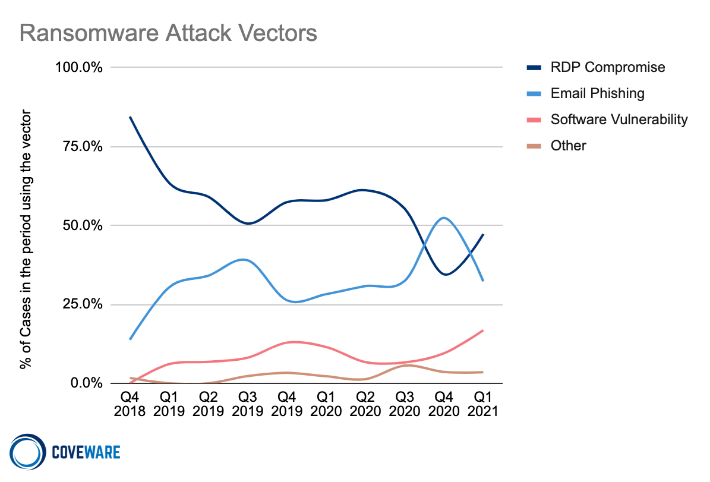
\includegraphics[width=0.77\linewidth]{figures/ransomware-attack-vectors.png}
	\caption{Wektory ataku ransomware  \cite{RansomwareAttackVectors}} 
	\label{Fig:Wektory ataku ransomware}
\end{figure} 

Jak można zauważyć, obecnie wiodącym źródłem dystrybucji tego złośliwego oprogramowania jest Remote Desktop Protocol (RDP) \cite{RDP} - protokół umożliwiający połączenie się z maszyną z systemem MS Windows, oraz przejęcie nad nim pełnej kontroli, używany w firmach jako narzędzie do konfiguracji urządzeń. 

Kolejno znajdują się e-maile phishingowe, opisane w poprzednim rozdziale. Ten sposób polega zazwyczaj na odpowiednim wykorzystaniu inżynierii społecznej, celem zmanipulowania ofiary do udzielenia poufnych danych dostępowych lub uruchomienia oprogramowania szyfrującego na swoim urządzeniu.  

Istotną regułą, którą należy się kierować przeciw tego typu złośliwemu oprogramowaniu w przedsiębiorstwie jest Zasada najmniejszego uprzywilejowania (ang. Principle of least privilege). Polega ona na zapewnieniu pracownikom dostępu tylko do tych zasobów, do których jest to konieczne przy wykonywaniu standardowej pracy. Ogranicza to dostęp do wrażliwych danych do minimum, co znacznie utrudnia infekcję najbardziej krytycznych elementów infrastruktury takich jak serwery produkcyjne, miejsca do przechowywania wrażliwych danych lub kopii zapasowych. 

Najlepszą metodą przeciwko tego  jest systematyczne wykonywanie archiwizacji danych. W sytuacji w której \emph{ransomware} trafi do komputera i zaszyfruje wszystkie pliki, pozostaje jedynie odtworzyć kopię zapasową. Dobrym sposobem jest także częste aktualizowanie systemu operacyjnego, celem eliminowania potencjalnych luk bezpieczeństwa.

\subsubsection{Implementacja}

Kurs ransomware rozpoczyna się od przedstawienia użytkownikowi podstawowych elementów związanych z tego typu atakiem, takich jak metody infekcji, generowanie kluczy szyfrujących czy sposoby ochrony przed ransomware. Użytkownicy o zaawansowanym typie konta mogą dowiedzieć się na temat działania filtrów antyspamowych, które stosowane są w zdecydowanej większości usług poczty elektronicznej.

Istotnym elementem kursu ransomware jest interaktywny slajd, który pozwala użytkownikowi na symulację pobrania złośliwego załącznika od nieznanego adresata w wirtualnym kliencie pocztowym w symulowanej przeglądarce internetowej. 

\begin{figure}[H]
	\centering
	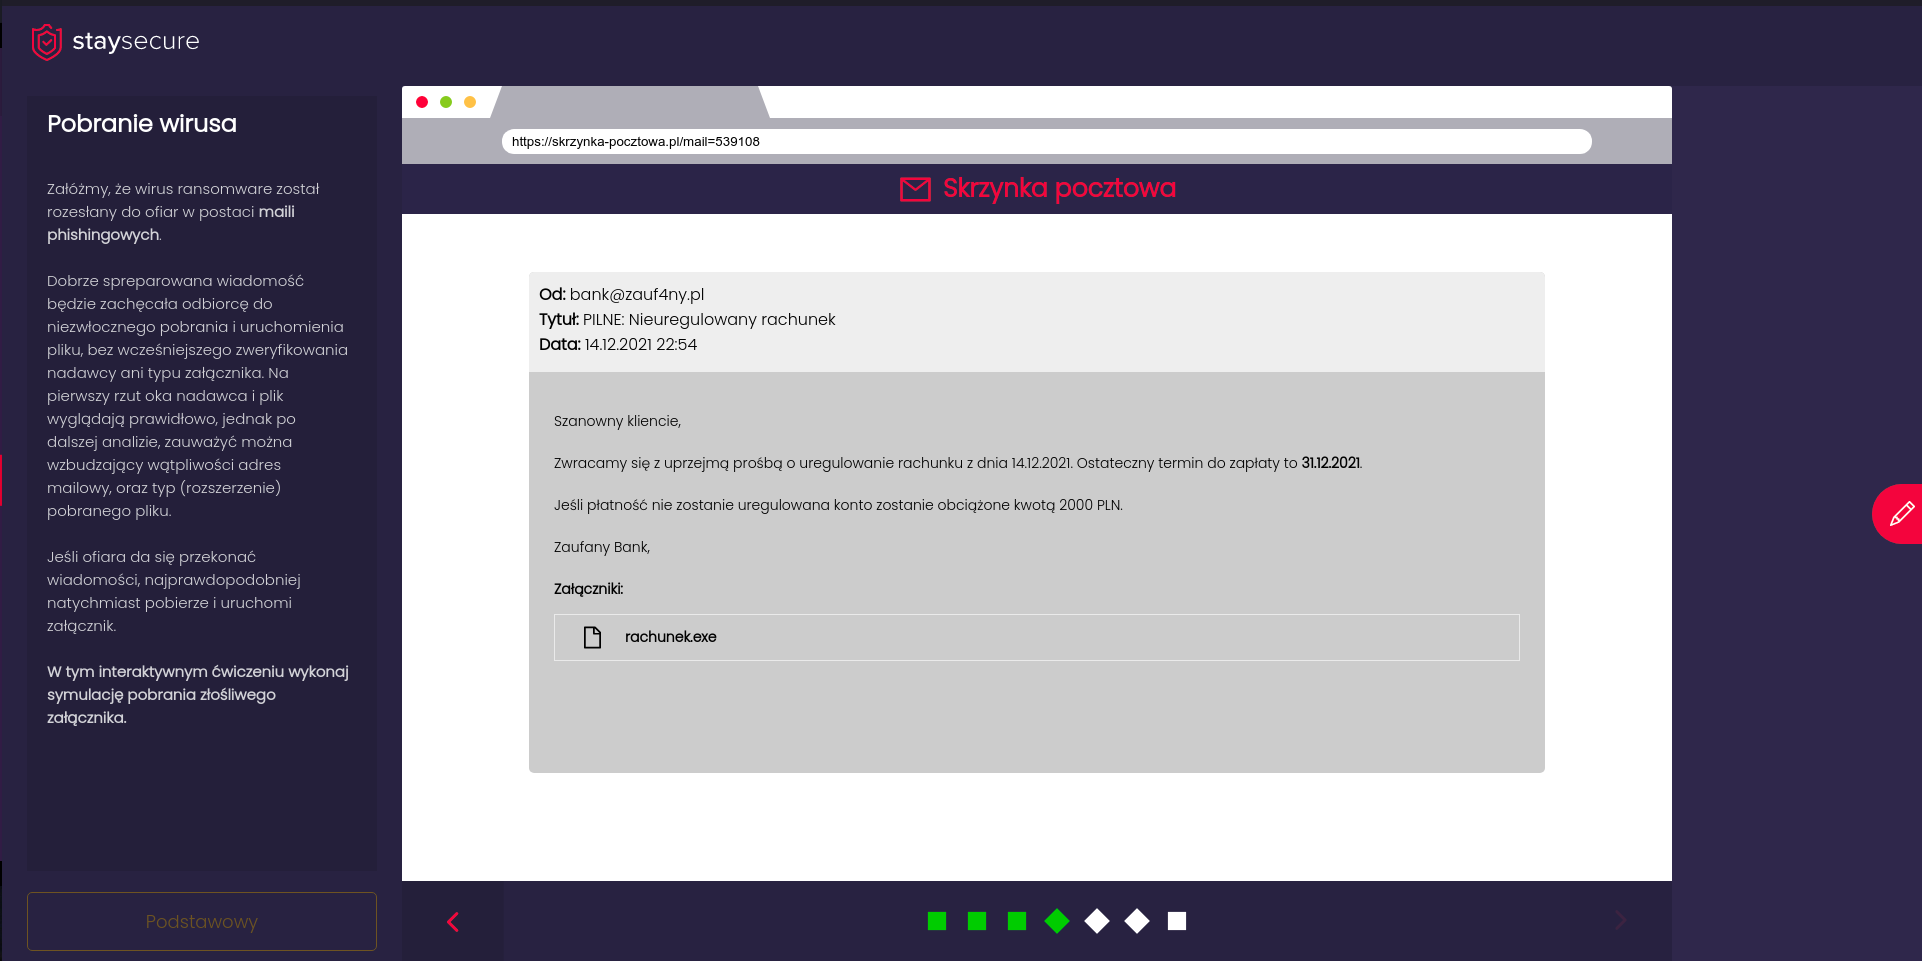
\includegraphics[width=0.99\linewidth]{figures/ransomware-slide-screenshot1}
	\caption{Interaktywny slajd przedstawiający sytuację pobrania ransomware. Źródło: opracowanie własne}
\end{figure}

Po pobraniu ransomware, kursantowi przedstawiony jest widok ekranu, na którym uruchomiony jest system Microsoft Windows 10. Warto zauważyć, że pobrany wcześniej załącznik znajduje się na liście plików w systemie, takich jak zdjęcia czy ważne dokumenty. Zadaniem użytkownika jest uruchomienie omawianego złośliwego pliku.

\begin{figure}[H]
	\centering
	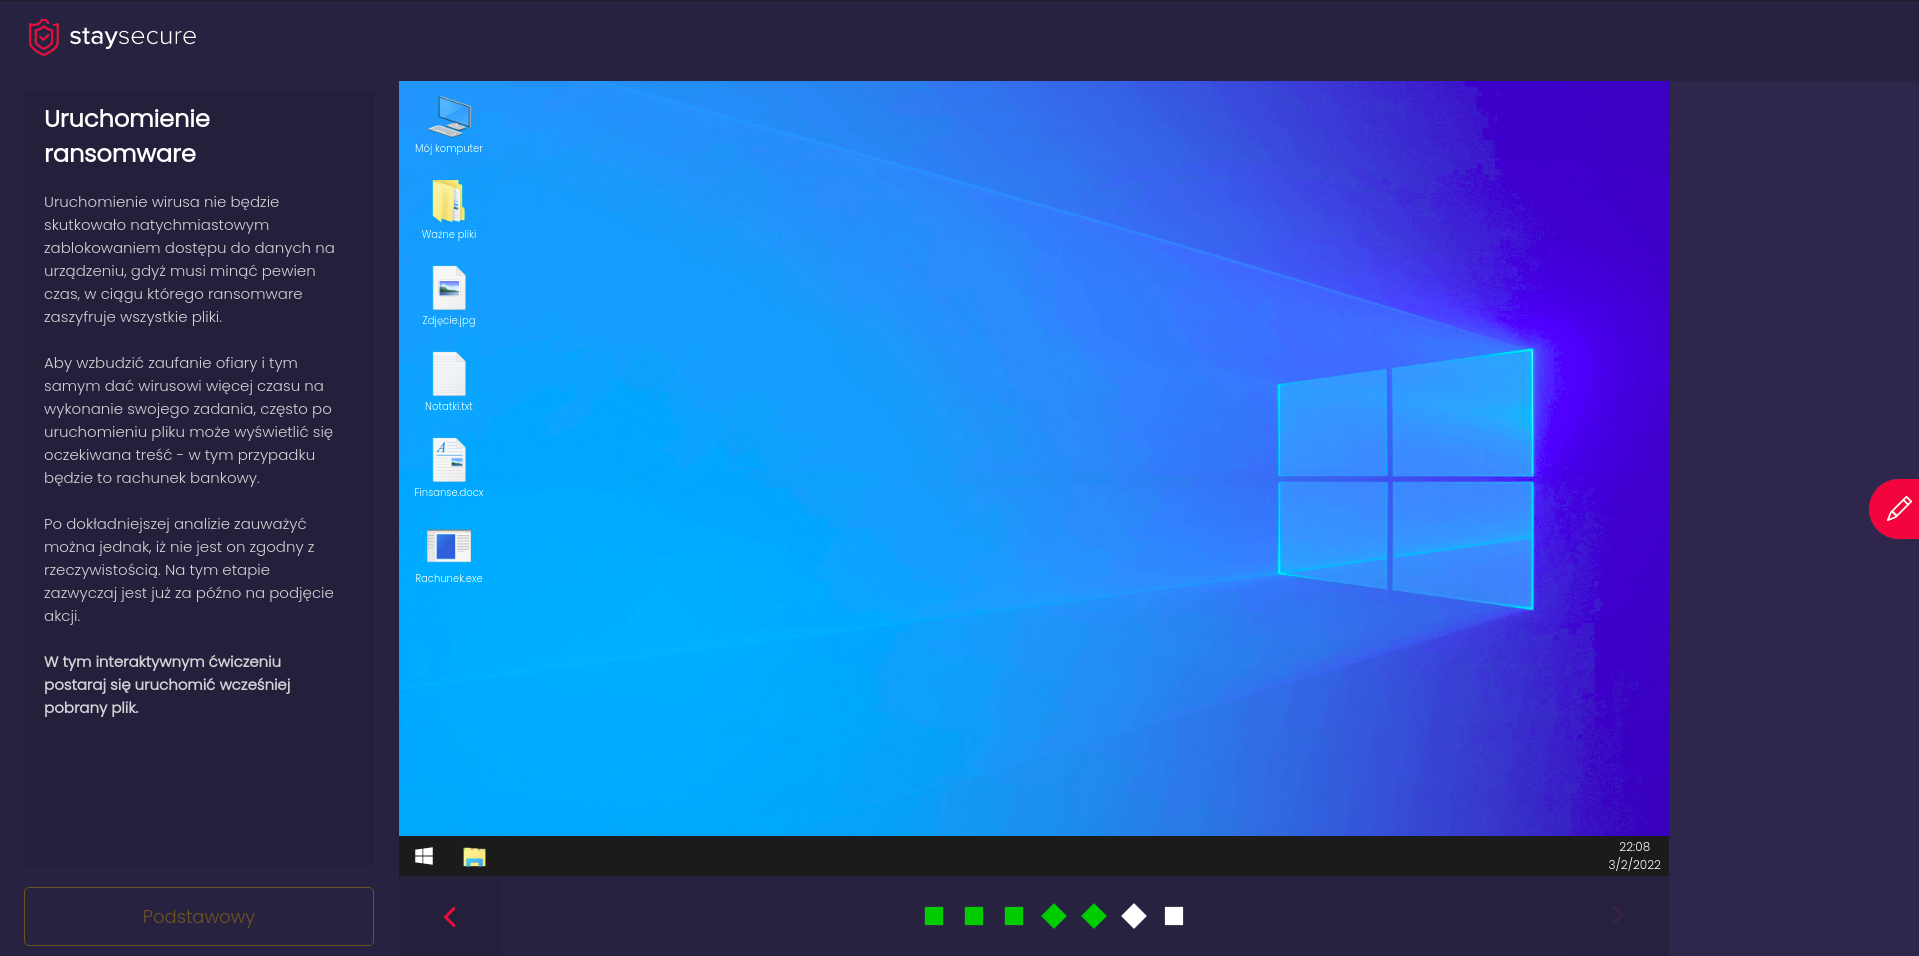
\includegraphics[width=0.99\linewidth]{figures/ransomware-slide-screenshot2}
	\caption{Interaktywny slajd przedstawiający widok urządzenia z systemem operacyjnym Microsoft Windows 10. Źródło: opracowanie własne}
\end{figure}

Zgodnie z opisem slajdu, uruchomienie ransomware będzie skutkowało rozpoczęciem szyfrowania wrażliwych plików na urządzeniu, jednak użytkownikowi przedstawiony zostanie fałszywy dokument. 

\begin{figure}[H]
	\centering
	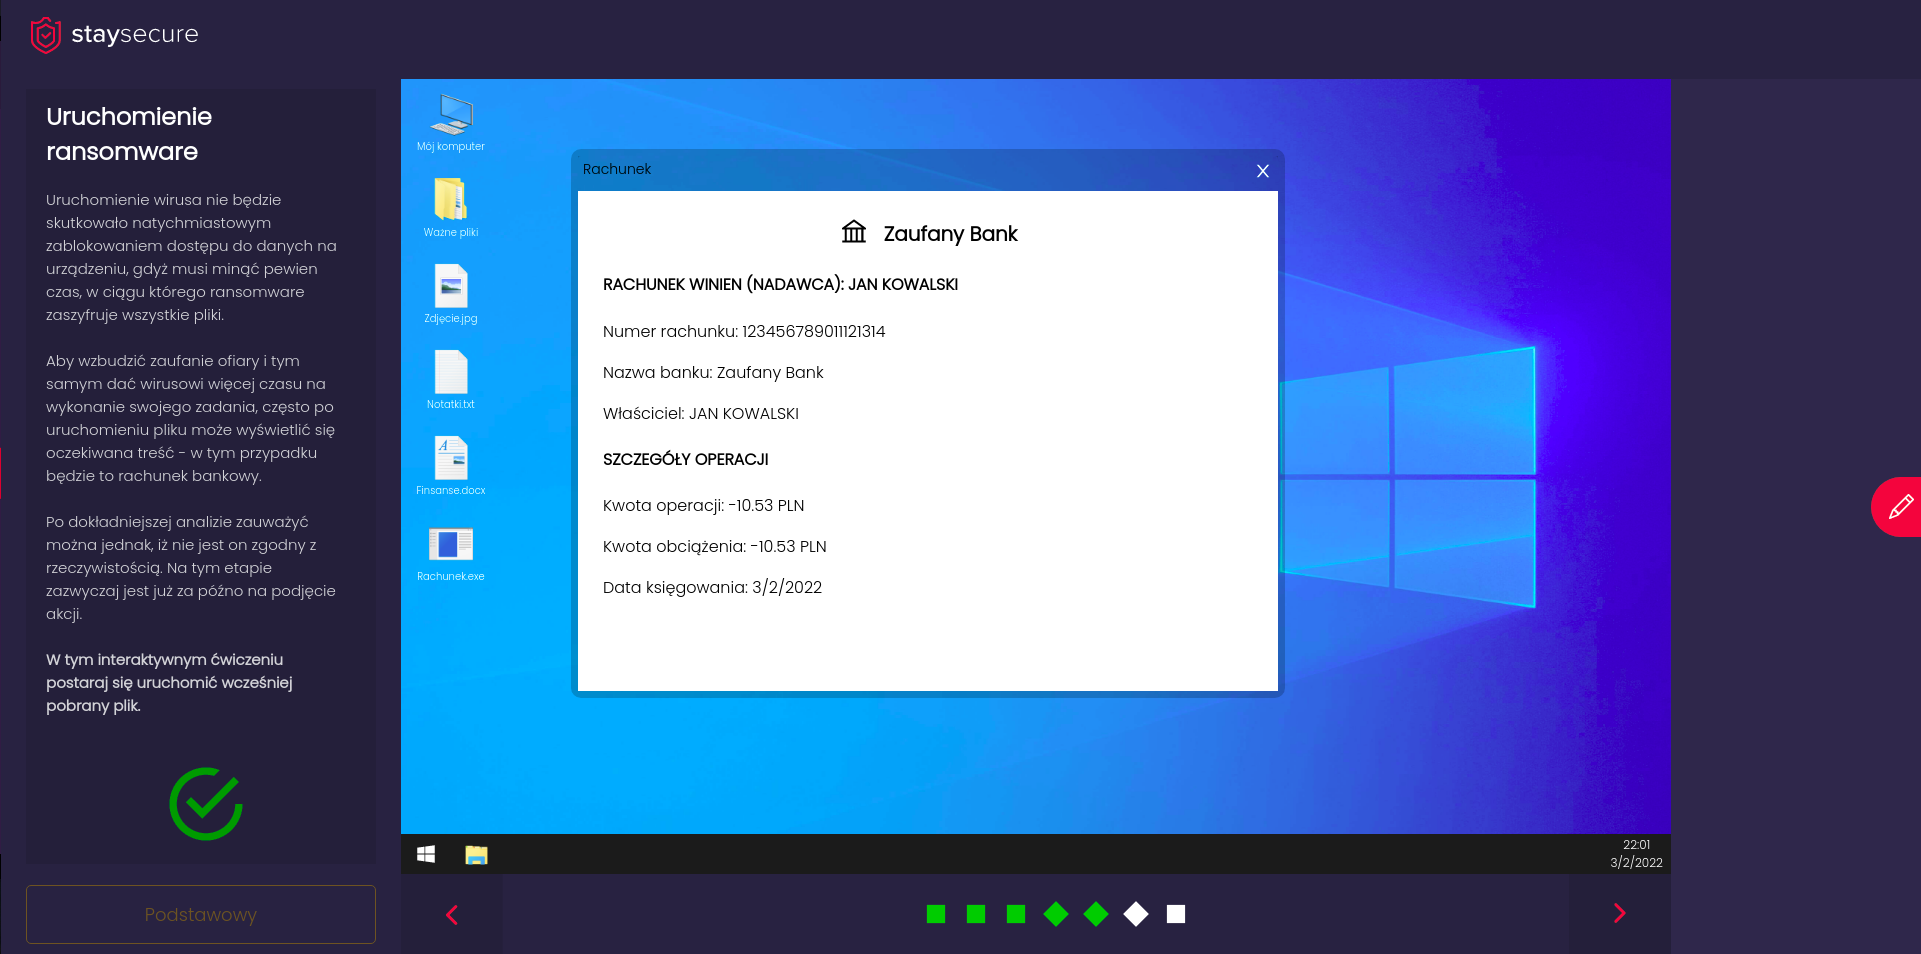
\includegraphics[width=0.98\linewidth]{figures/ransomware-slide-screenshot3}
	\caption{Interaktywny slajd przedstawiający widok urządzenia z systemem operacyjnym Microsoft Windows 10. Źródło: opracowanie własne}
\end{figure}

W kolejnym slajdzie zauważyć można, że wszystkie ważne dokumenty na urządzeniu zostały zaszyfrowane, oraz uruchomione zostało okno ransomware.


\begin{figure}[H]
	\centering
	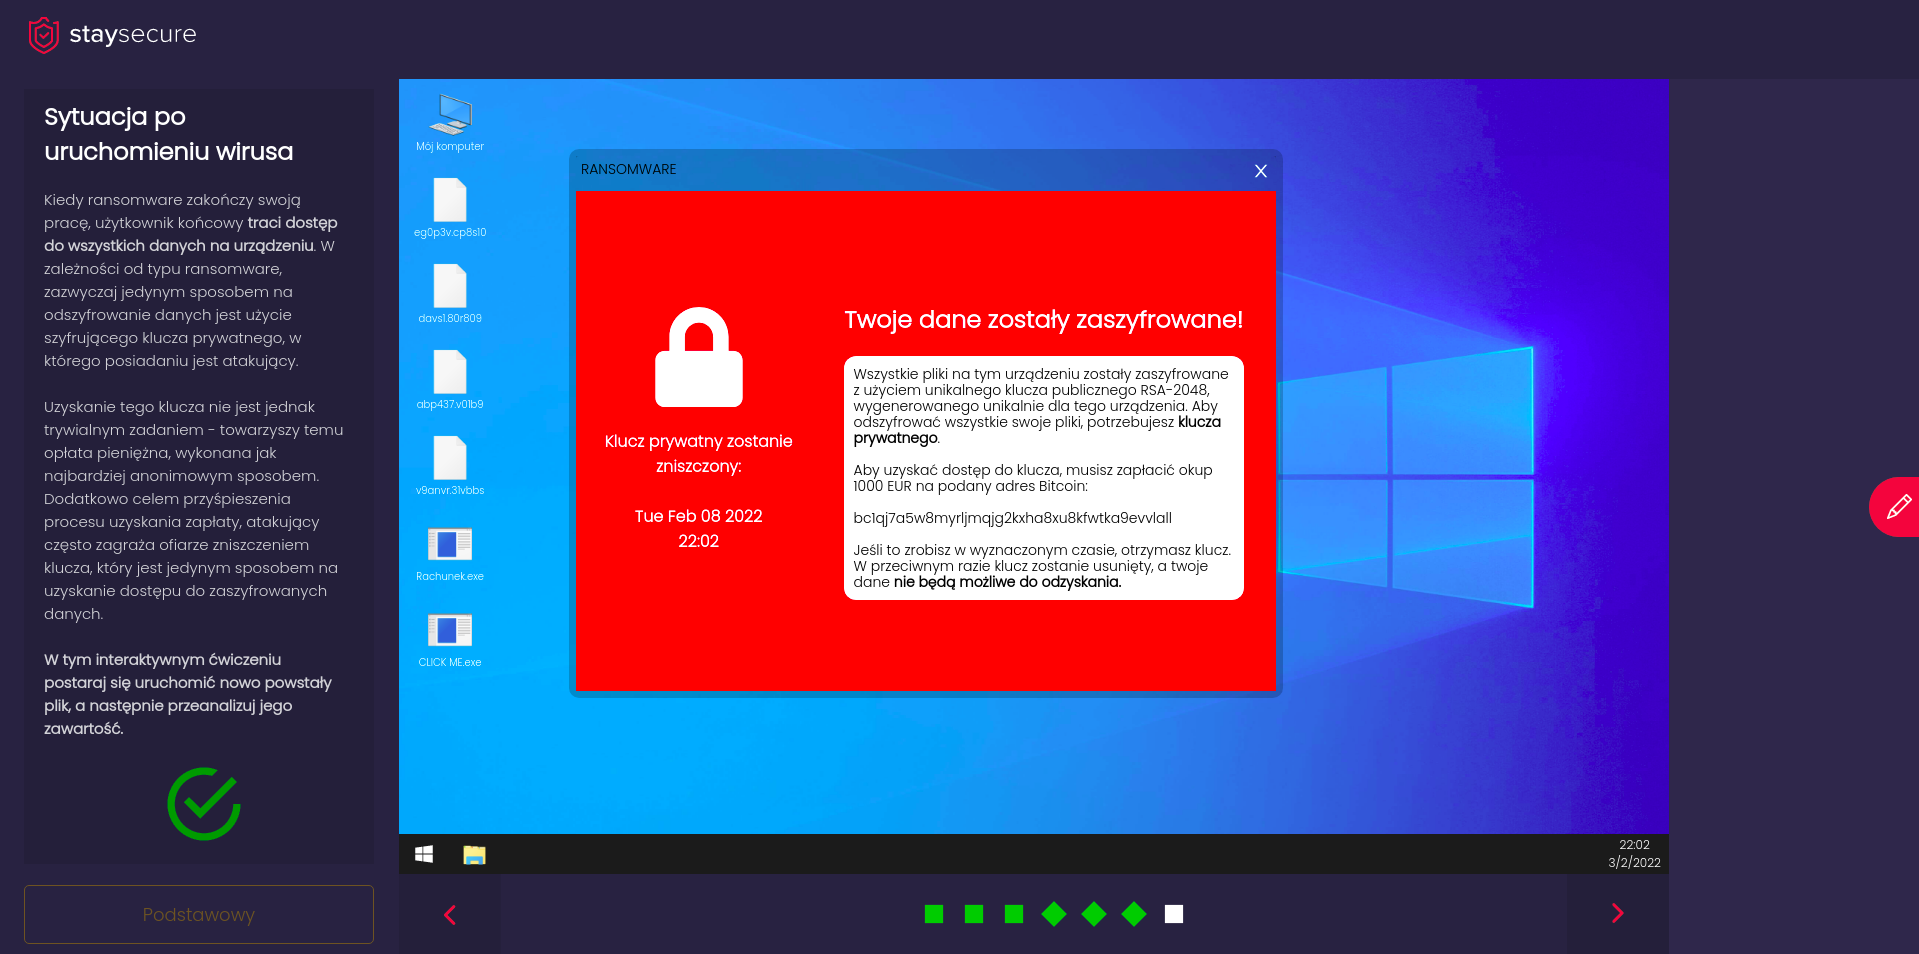
\includegraphics[width=0.98\linewidth]{figures/ransomware-slide-screenshot4}
	\caption{Interaktywny slajd przedstawiający widok po uruchomieniu ransomware. Źródło: opracowanie własne}
\end{figure}

Poprzez możliwie najlepsze odwzorowanie codziennych warunków, z którymi kursant może mieć do czynienia, efekty infekcji ransomware mogą być dużo bardziej przystępne do zrozumienia, niż opis w formie pisemnej. Interaktywne slajdy pozwalają kursantowi wczuć się w role ofiary, dzięki czemu będzie w stanie bezpiecznie zainfekować urządzenie ransomware. 

\clearpage
\subsection{Blokada usług}
\subsubsection{Opis}
Celem Blokady usług (DOS) są zazwyczaj serwisy internetowe małych i średnich przedsiębiorstw. Atak ten polega na wykonaniu tak wielu żądań do serwera w jednostkowym czasie, aby ten przestał odpowiadać. Są relatywnie proste w wykonaniu i mogą być powodem poważnych strat dla sieci i systemów komputerowych. Większa część ataków typu \emph{Flood} odbywa się w oparciu o luki w protokole TCP, co prowadzi do takich ataków jak \emph{TCP SYN Flood DoS} \cite{Ddos}.

Rodzaj DOS może różnić się w zależności od warstwy modelu OSI, na której wysyłane są pakiety. Do głównych rodzajów tego ataku zaliczyć można: SYN Flood, HTTP Flood, Smurf Attack. W momencie, w którym klient chce nawiązać połączenie z serwerem, obie maszyny sekwencyjnie wymieniają zestaw komunikatów, znany także jako uzgadnianie trój-etapowe - \emph{3-Way Handshake} \cite{3WayHandshake}. 

\begin{enumerate}
	\item W pierwszym kroku klient wysyła segment z SYN (ang. Synchronize Sequence Number), który informuje serwer, że klient prawdopodobnie rozpocznie komunikację i z jakim numerem sekwencyjnym uruchamia segmenty.
	\item Kolejno serwer odpowiada na żądanie klienta z ustawionymi bitami sygnału SYN-ACK. Potwierdzenie (ACK) to odpowiedź segmentu, który otrzymał, a SYN oznacza, z jakim numerem sekwencji prawdopodobnie rozpoczną się segmenty.
	\item W końcowej części klient potwierdza odpowiedź serwera i oboje ustanawiają połączenie, w którym rozpocznie rzeczywisty transfer danych.
\end{enumerate}


\begin{figure}[H]
	\centering
	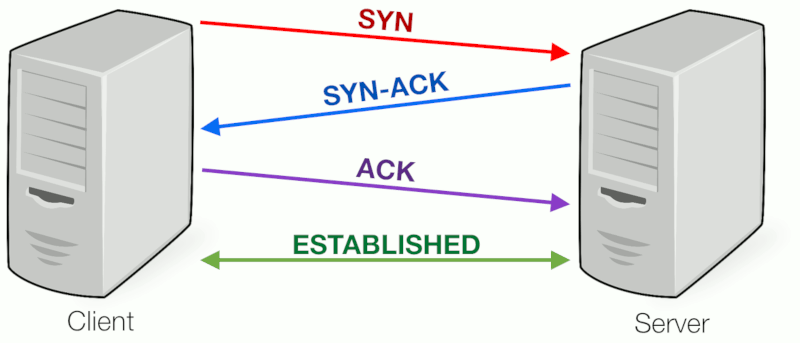
\includegraphics[width=0.7\linewidth]{figures/3-way-handshake}
	\caption{Graficzna reprezentacja uzgadniania trój-etapowego \cite{ThreeWayHandshakePicture}}
	\label{fig:3-way-handshake}
\end{figure}

\emph{SYN Flood} polega na nadużyciu wyżej opisanej procedury. Atakujący przesyła do serwera falę komunikatów SYN, używając spreparowanych adresów IP. Niczego nieświadomy serwer odpowiada na żądania komunikatem SYN-ACK, po czym oczekuje na odpowiedź ACK od klienta celem sfinalizowania uzgodnienia trój-etapowego. Ze względu na fakt, iż serwer oczekuje na zakończenie komunikatu z fałszywymi adresami IP, połączenie to nigdy nie dojdzie do skutku. Efektem tego jest przeładowanie kolejki połączeń i ostatecznie pamięci operacyjnej serwera, powodując brak odpowiedzi na żądania zwykłych użytkowników \cite{DDosHowItWorks}. 

Blokada danego adresu IP, z którego przychodzi wiele żądań w krótkim okresie czasu, nie stanowi większego problemu dla firewalli (zapór ogniowych), dlatego też coraz powszechniejszymi stają się ataki DDOS - \emph{Distributed Denial-Of-Service}. Różnica polega na tym, że żądania wysyłane są z wielu lokacji jednocześnie, co znacznie bardziej utrudnia identyfikację i zablokowanie nagłego ruchu przez zaporę ogniową.

Szybka detekcja nienaturalnego obciążenia serwera ma kluczowe znaczenie dla ochrony przed atakiem DDOS. W przypadku przedsiębiorstw wiąże się to także z zapewnieniem akceptowalnej jakości usług dla klientów oraz stratami, spowodowanymi niedostępnością serwisu. Istnieje wiele rozwiązań, które pozwalają wykrywać powyżej opisany incydent. Można je podzielić według sposobu ich działania i złożoności wykrywania. Do najskuteczniejszych rozwiązań należy analiza statystyczna ruchu, logika rozmyta, stosowanie sztucznych sieci neuronowych czy techniki eksploracji ukrytych zależności w repozytoriach danych \cite{DDosDetection}. 

Ataki \emph{Denial of Service} stanowią zdecydowanie większe zagrożenie dla klasycznego modelu hostingu strony webowej, w którym celem zapewnienia dostępności serwisu korzysta się z fizycznych serwerów. W sytuacji, w której obciążenie aplikacji wzrośnie, przykładowo na skutek omawianego ataku, jedynym rozwiązaniem jest filtrowanie i odrzucanie potencjalnych złośliwych żądań - nie ma opcji na szybkie zwiększenie zasobów. 

W dzisiejszych czasach zdecydowanie lepszym rozwiązaniem zarówno pod kątem finansowym, jak i prostoty są publiczne chmury obliczeniowe, takie jak AWS (ang. Amazon Web Services), Microsoft Azure lub GCP (ang. Google Cloud Platform). Ich bogata oferta zapewnia podstawowe usługi takie jak dedykowane serwery, wirtualne sieci i interfejsy sieciowe czy usługi przechowywania danych. Ponadto chmury oferują usługi zaawansowanych mechanizmów przeciwdziałania atakom typu DDOS. Przykładem może być funkcjonalność chmury AWS w postaci grupy auto-skalującej (ang. auto-scaling group). Usługa ta dostosowuje liczbę instancji serwerowych w zależności od aktualnie panującego ruchu. Tak więc przy normalnych warunkach, gdy obciążenie serwera jest na niskim poziomie, w grupie może znajdować się jedna instancja serwerowa. Gdy tylko określony zasób przekroczy wcześniej zadeklarowaną wartość, na przykład zasoby procesora osiągną 80\% dostępnych zasobów w okresie minuty, automatycznie zostanie stworzona kolejna instancja serwerowa na podstawie pierwotnej. Tym samym ruch sieciowy zostanie rozłożony pomiędzy dwa serwery, zamiast jednego. 

Dobrym rozwiązaniem na tego typu ataki może być również użycie systemu równoważenia obciążenia - \emph{load balancera}. Jest to mechanizm, wykorzystywany w serwisach internetowych korzystających z większej ilości instancji serwerowych. W rezultacie każde połączenie jest przekierowane do jednego z dostępnych serwerów według następujących algorytmów:
\begin{itemize}
	\item \emph{Round Robin} - nadchodzące żądanie zostanie przekierowane do każdego serwera po kolei. Gdy dojdzie do końca, zrestartuje się.
	\item \emph{Least Connections} - \emph{Load Balancer} prześle żądanie do jednego z serwerów, które aktualnie procesują najmniejszą ilość żądań.
	\item \emph{IP Hash} - żądanie zostanie skierowane do najbliższego serwera pod kątem geolokalizacji. 
\end{itemize}

Ataki DOS są bezpośrednim zagrożeniem dla dostępności aplikacji webowych. Jeśli złośliwy ruch jest odpowiednio duży i nie zostanie szybko zidentyfikowany, może z łatwością przyczynić się do wyłączenia strony internetowej na nieokreślony czas. Dzięki wielu łatwo dostępnym narzędziom, takim jak systemy równoważenia obciążenia, grupy auto-skalujące, firewalle, ochrona przed tego typu zagrożeniem stała się dużo łatwiejsza niż kiedykolwiek.

\subsubsection{Implementacja}

Kurs o tematyce blokady usług przedstawia użytkownikowi podstawowe koncepty związane z działaniem serwerów webowych oraz atakami typu DOS/DDOS. Poprzez slajdy obrazujące natężenie ruchu przykładowego serwera, kursant jest w stanie w łatwy sposób zwizualizować sobie okoliczności i skutki omawianego ataku.

\begin{figure}[H]
	\centering
	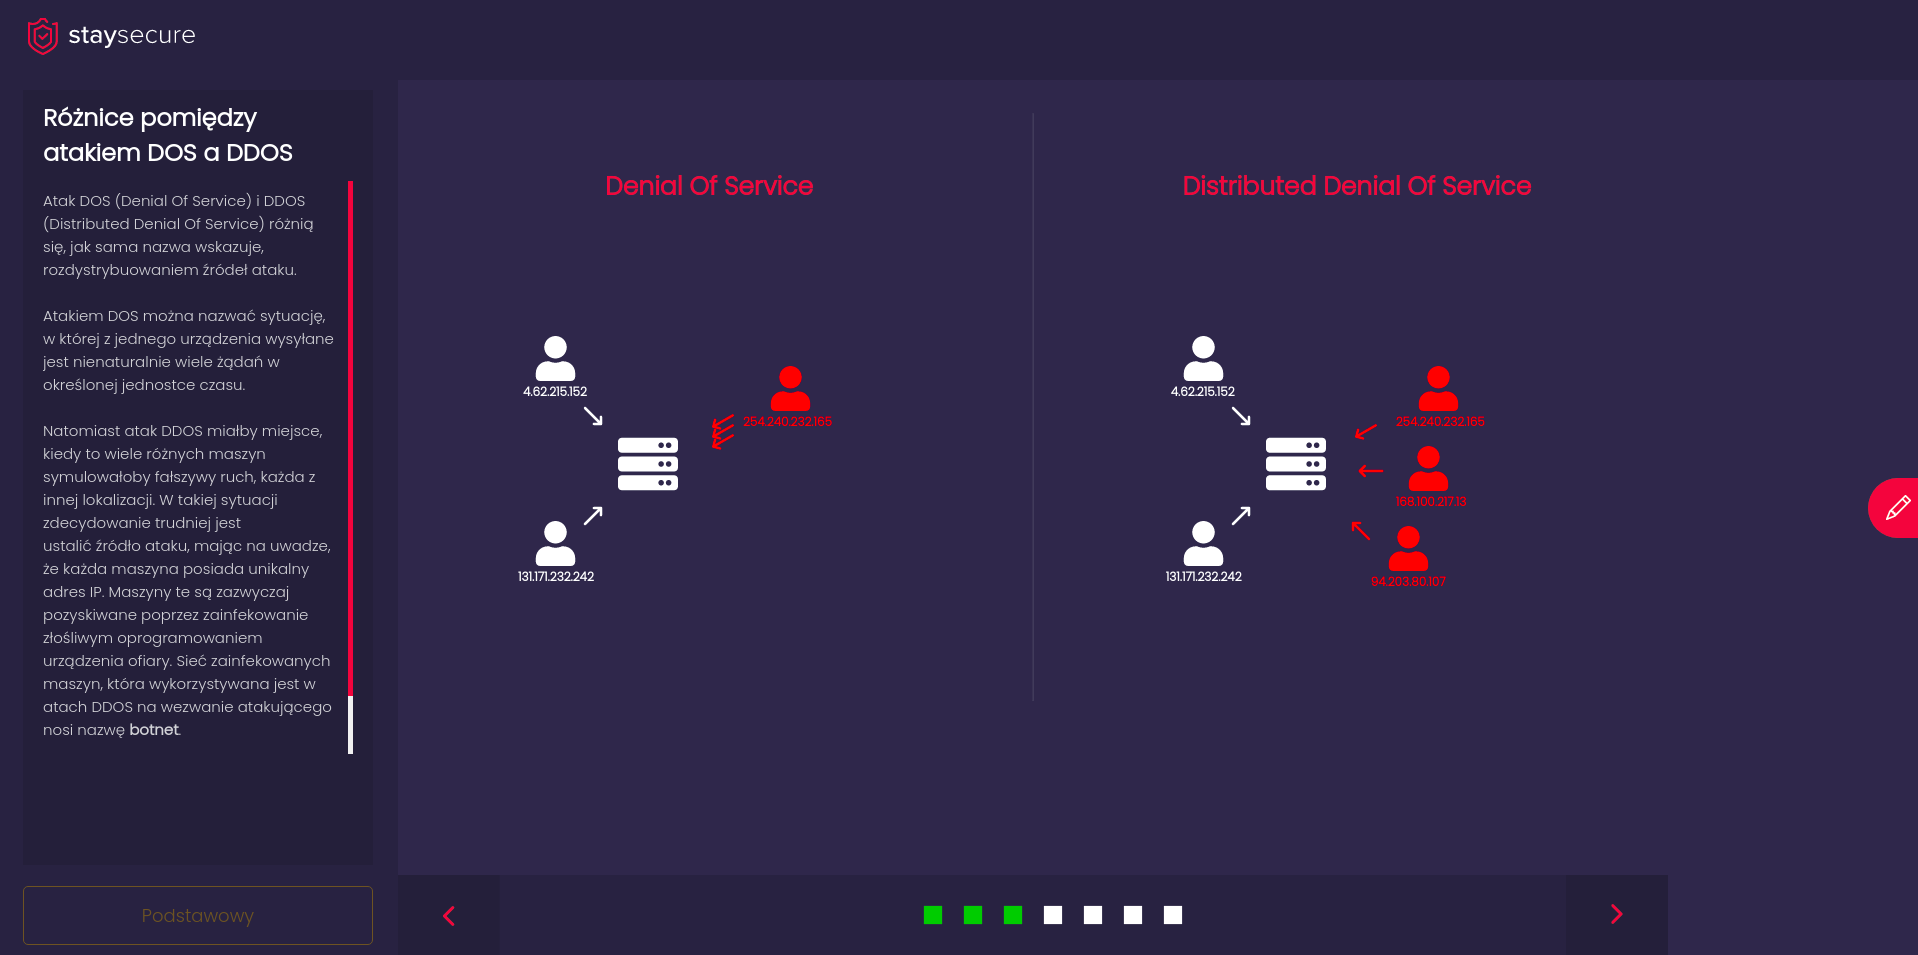
\includegraphics[width=0.99\linewidth]{figures/dos-slide-screenshot1}
	\caption{Slajd przedstawiający różnicę pomiędzy atakiem DOS a DDOS. Źródło: opracowanie własne}
\end{figure}

Szczegółowo omawiane są także typy ataków DDOS i metody ochrony przeciw nim.
Pozwala to kursantowi na dostrzeżenie skali niebezpieczeństwa, poprzez fakt, że ataki DDOS mogą występować na wielu różnych poziomach, często niezależnych od siebie oraz możliwości łączenia typów ataku

\begin{figure}[H]
	\centering
	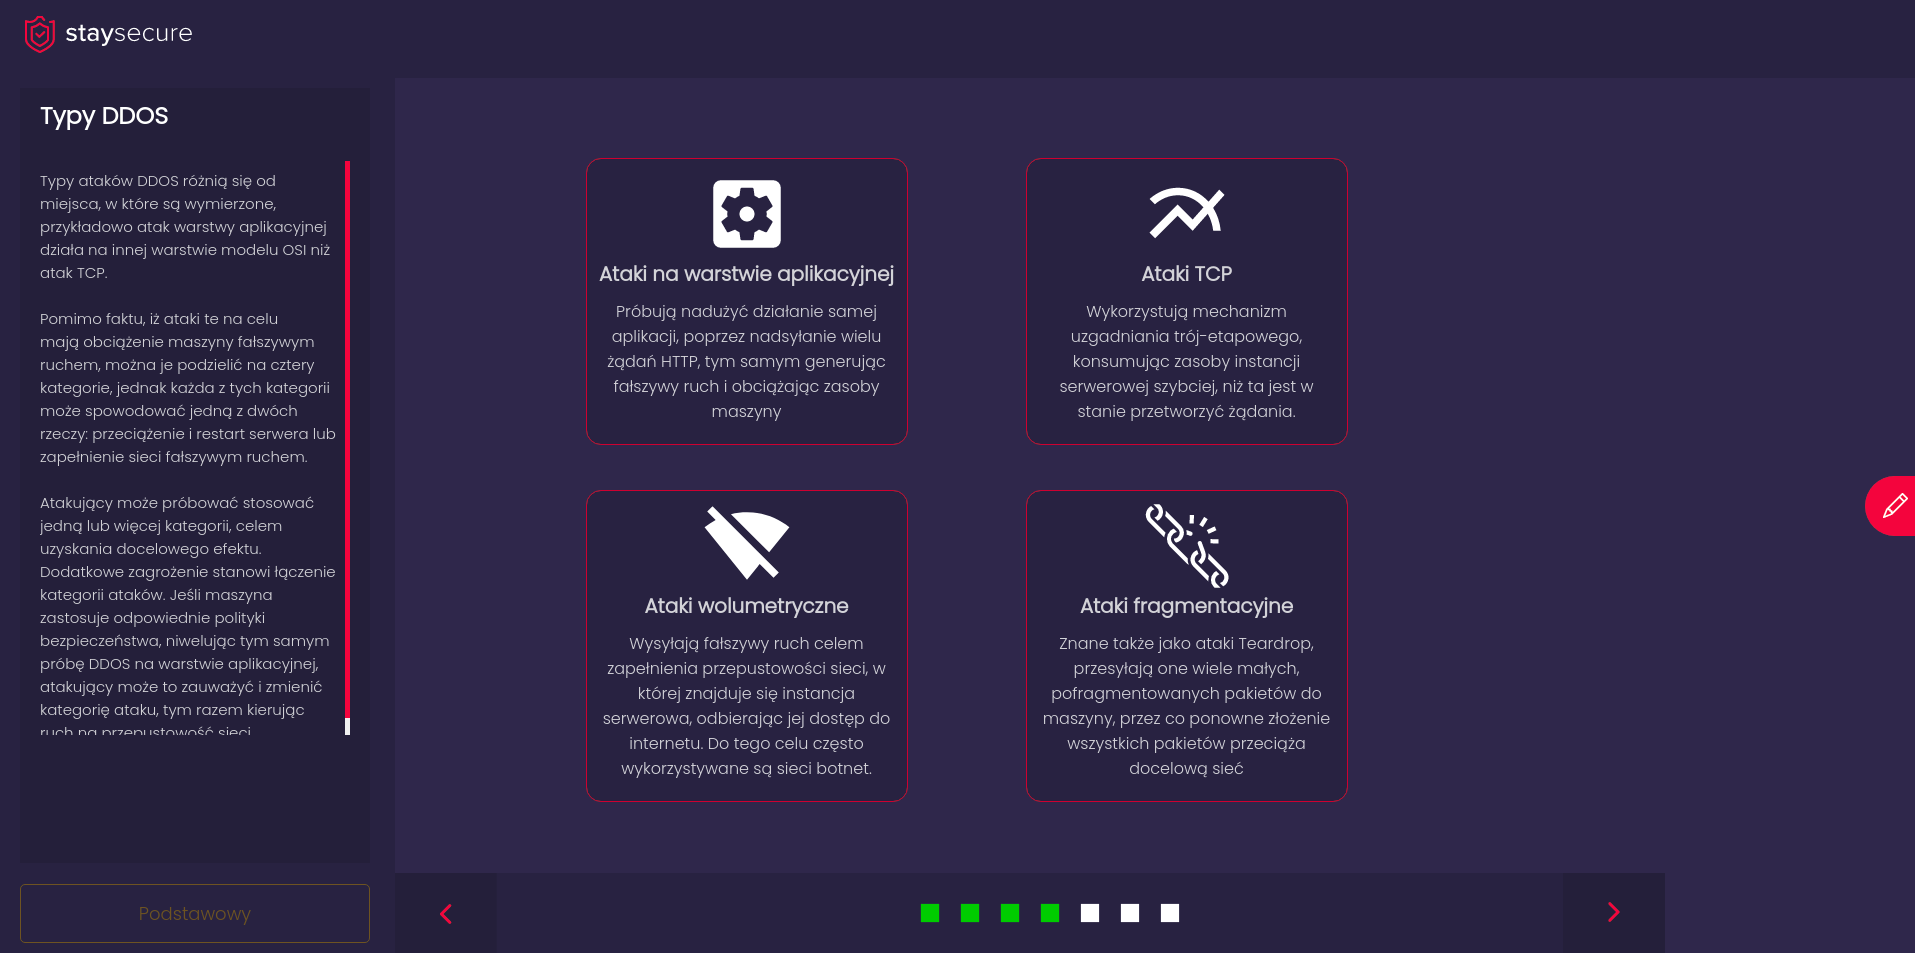
\includegraphics[width=0.99\linewidth]{figures/dos-slide-screenshot2}
	\caption{Slajd przedstawiający typy ataków DDOS. Źródło: opracowanie własne}
\end{figure}

Użytkownicy o zaawansowanym typie konta mogą dowiedzieć się o metodach ochrony przeciw atakom DDOS, które w dzisiejszych czasach są stosowane przez zdecydowaną większość usług hostingowych. 

\begin{figure}[H]
	\centering
	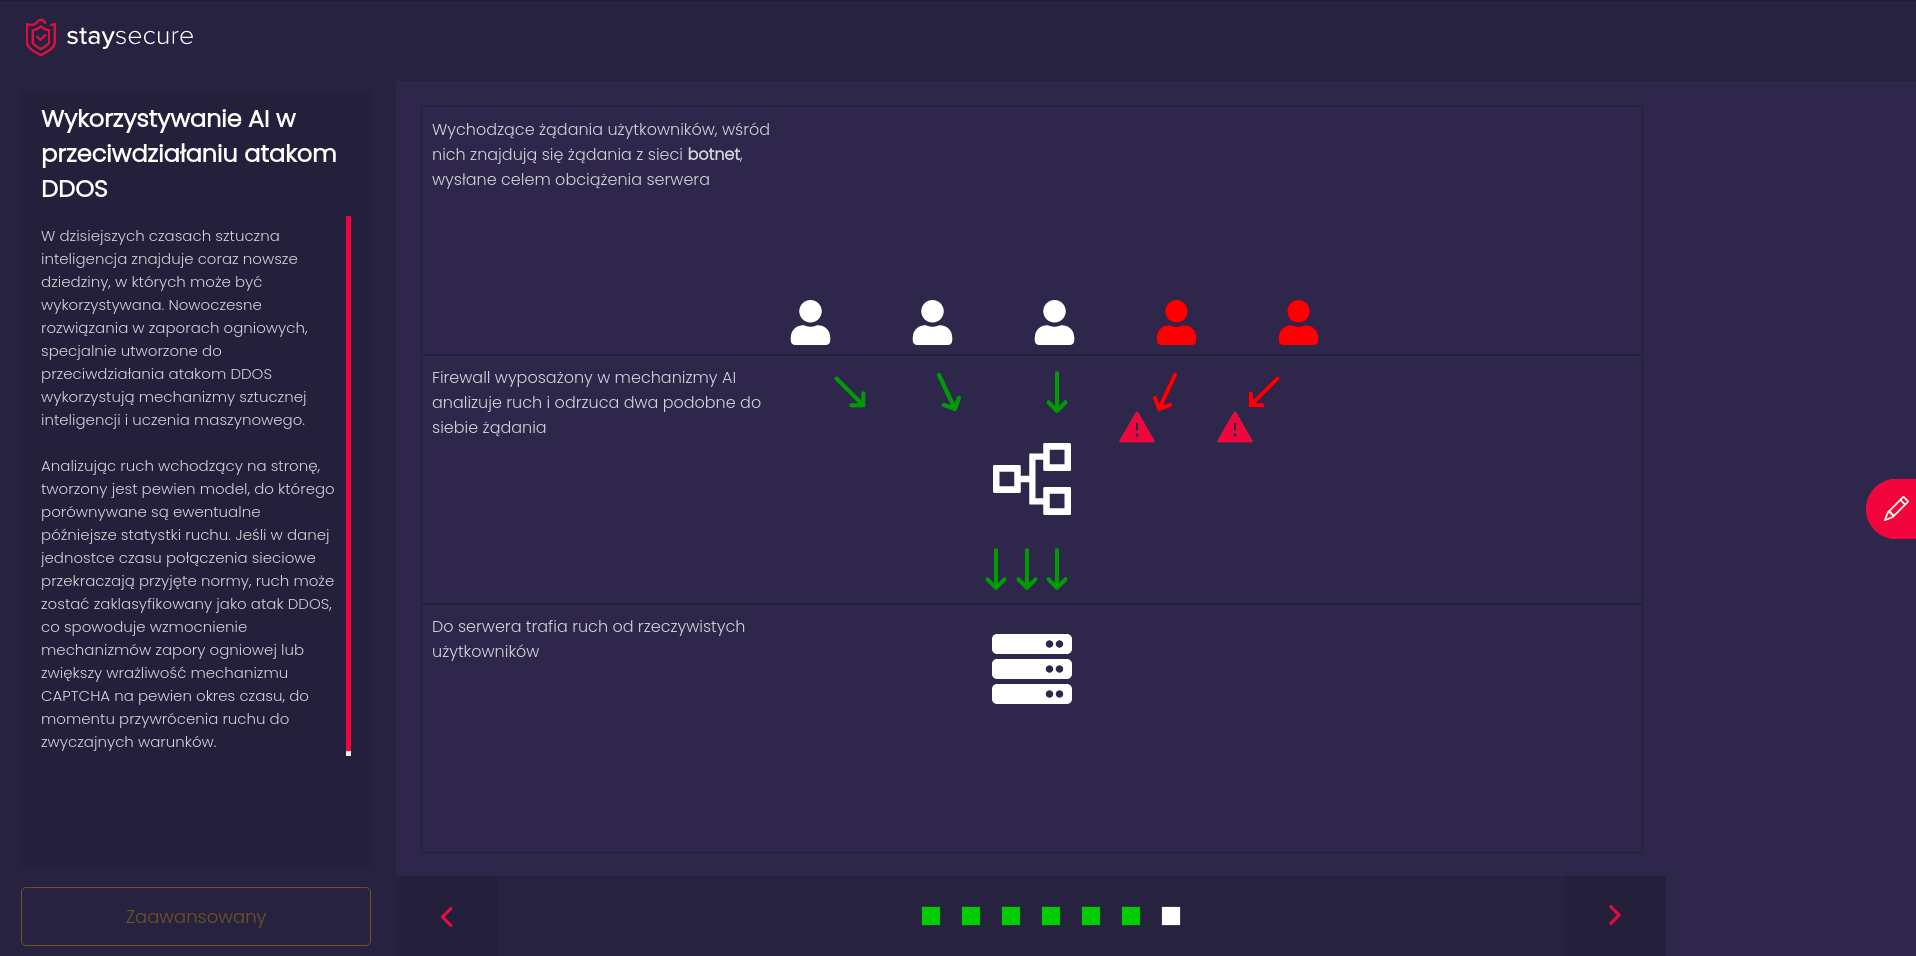
\includegraphics[width=1\linewidth]{figures/dos-slide-screenshot3}
	\caption{Slajd przedstawiający sposoby wykorzystania sztucznej inteligencji w ochronie przed atakami DDOS. Źródło: opracowanie własne}
\end{figure}


W ramach rozbudowy projektu zawartość kursu może zostać rozszerzona o dodatkowe elementy, które pozwolą użytkownikowi na przeprowadzenie symulacji ataku DDOS, w którym będzie mógł zauważyć, że strona, która do tej pory działała, po uruchomieniu symulowanego ataku jest niedostępna.
 
\clearpage


\subsection{Keylogger}
\subsubsection{Opis}
Keylogger to całkowicie legalne narzędzie rejestrujące zdarzenia związane z obsługą klawiatury systemu operacyjnego, na którym się znajduje, zazwyczaj bez wiedzy użytkownika. Pierwsze keyloggery powstały w latach 70 XX wieku i miały służyć służbom specjalnym do przechwytywania informacji na maszynach do pisania w publicznych miejscach.

To narzędzie może być wykorzystywane w miejscach pracy do badania aktywności pracowników, jako rodzaj kontroli rodzicielskiej lub przez oszustów próbujących wykraść wrażliwe dane ofiary. Ich celem jest zazwyczaj zarejestrowanie aktywności klawiatury użytkownika i przechwycenie tych informacji, celem wydobycia takich danych jak dane uwierzytelniające czy numery kart kredytowych.

Keyloggery mogą dzielić się na:

\begin{itemize}
	\item sprzętowe, przypominają pamięci przenośne (pendrive). Podłączane do urządzenia zazwyczaj poprzez interfejs USB, jednak mogą występować jako urządzenie pośredniczące pomiędzy klawiaturą a złączem USB komputera. Ich zaletą jest obszar działania - potrafią rejestrować aktywność, nawet jeśli użytkownik nie uruchomił systemu operacyjnego i co do zasady potrafią być cięższe w detekcji dla antywirusa.
	\item programowe, są formą oprogramowania działającego w tle. Dostają się na urządzenie poprzez zainstalowanie programu. W zależności od celu keyloggera (miejsce pracy, kontrola rodzicielska, wirus), może on maskować swoją obecność, utrudniając tym samym detekcję. Podstawową funkcją tego programu jest przejmowanie kontroli nad procedurami związanymi z obsługą klawiatury systemu operacyjnego, na którym się znajduje.
\end{itemize}

Wraz z biegiem czasu, zaczęto nadużywać to narzędzie, stosując je do złośliwych celów. Obecnie, częstym zastosowaniem keyloggerów jest infekcja, a wykradanie wrażliwych danych, takich jak dane bankowe, kart kredytowych czy loginy i hasła. Do bardziej zaawansowanych funkcji keyloggera może należeć przechwytywanie ekranu zainfekowanej ofiary, poprzez tworzenie zrzutów ekranu, lub przechwytywanie skopiowanych informacji. Keyloggery stanowią wyjątkowe zagrożenie dla przedsiębiorstw - wykradzione dane mogą zapewnić dostęp atakującemu do najbardziej wrażliwych elementów przedsiębiorstwa lub wyjawić konfidencjonalne plany firmy.

Urządzenie może zostać zainfekowane keyloggerem na wiele sposobów, które różnią się w zależności od rodzaju tego narzędzia. Keyloggery sprzętowe, jak sama nazwa wskazuje, zazwyczaj wymagają fizycznej obecności atakującego przy sprzęcie ofiary, celem podłączenia keyloggera do urządzenia. W związku z tym stanowią one mniejsze zagrożenie dla zwykłych użytkowników niż keyloggery programowe.

Infekcja keyloggerem programowym jest znacznie prostsza, przez co ogólnie rzecz biorąc stanowi on większe zagrożenie, szczególnie jeśli urządzenie nie jest chronione antywirusem. Najczęstszą formą instalacji tego rodzaju złośliwego oprogramowania jest pobranie i uruchomienie podejrzanego załącznika z sieci lub z wiadomości phishingowych.

\subsubsection{Implementacja}

W kursie związanym z opisywanym zagrożeniem użytkownicy mogą dowiedzieć się informacji na temat historii keyloggerów, typami tego narzędzia oraz stosowaniem go do złośliwych celów. Kursanci mogą także zaznajomić się z procesem detekcji zagrożenia na wirtualnym ekranie, na którym uruchomiony jest system Microsoft Windows 10. 

\begin{figure}[H]
	\centering
	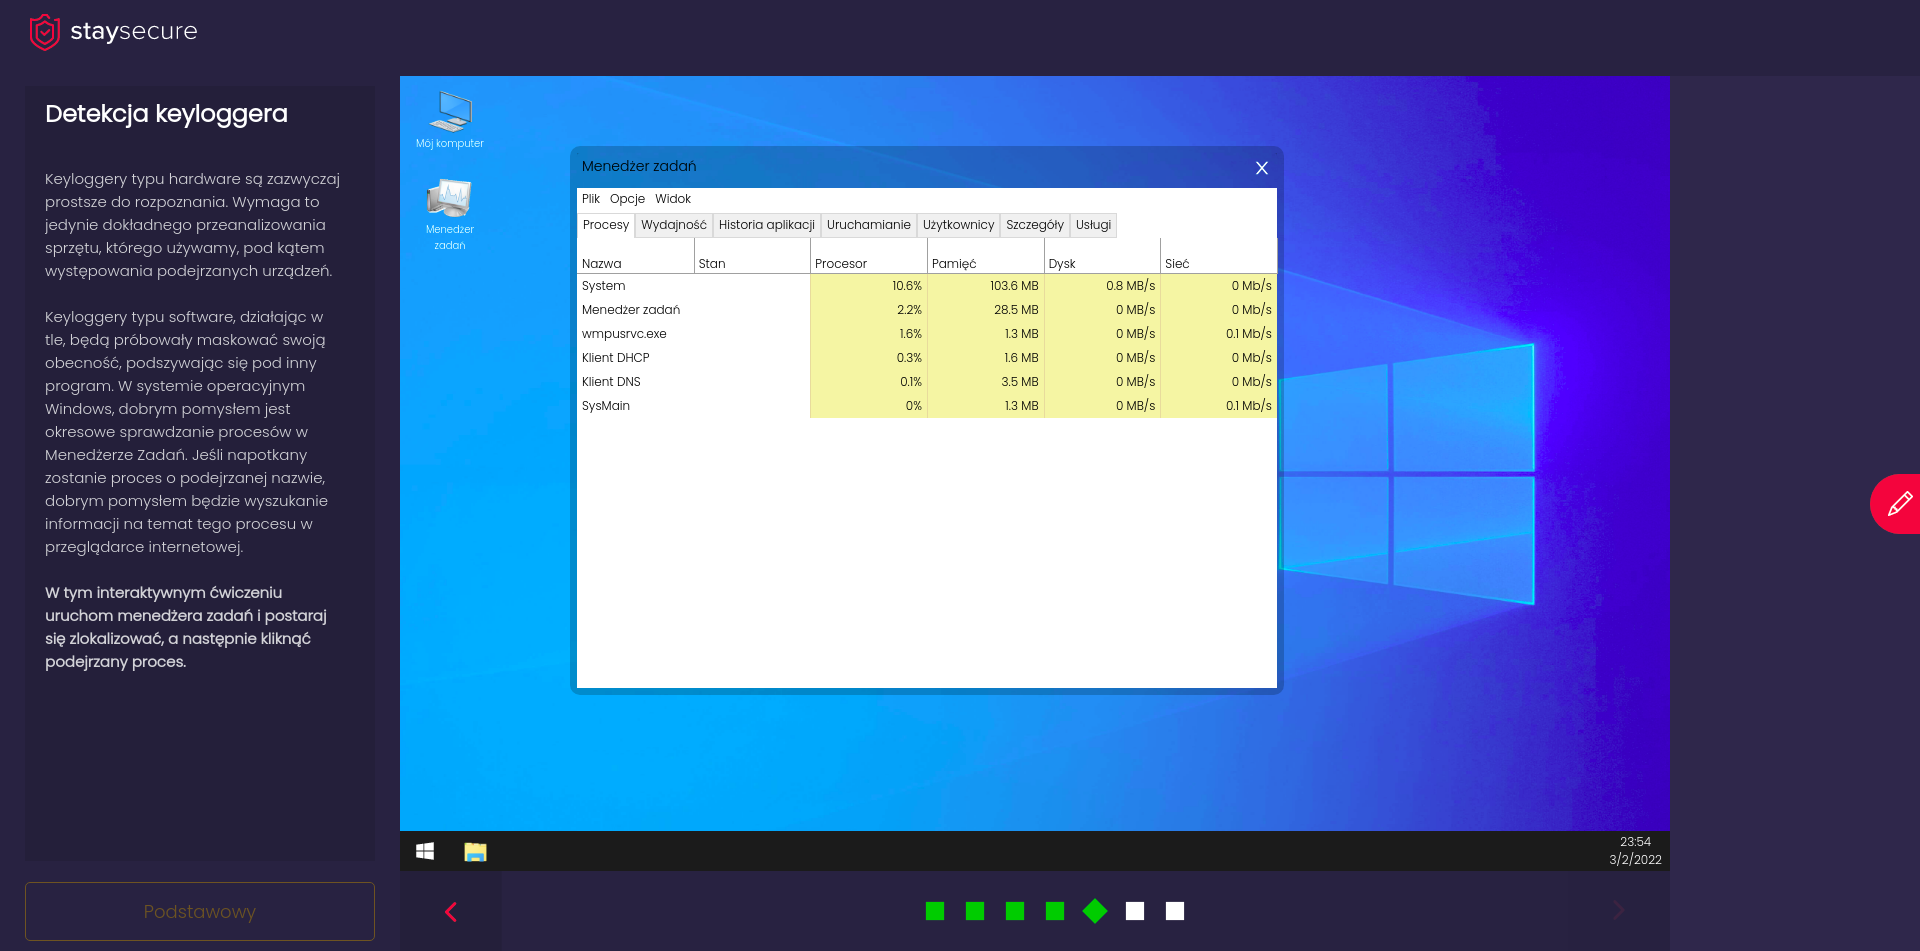
\includegraphics[width=1\linewidth]{figures/keylogger-slide-screenshot1}
	\caption{Interaktywny slajd przedstawiający aktualnie działające procesy w wirtualnym systemie. Źródło: opracowanie własne}
\end{figure}

Kursanci mogą również zdobyć informacje na temat metod ochrony przed tego typu atakiem, korzystając między innymi z menedżerów haseł, uwierzytelniania dwuskładnikowego czy antywirusa.

\begin{figure}[H]
	\centering
	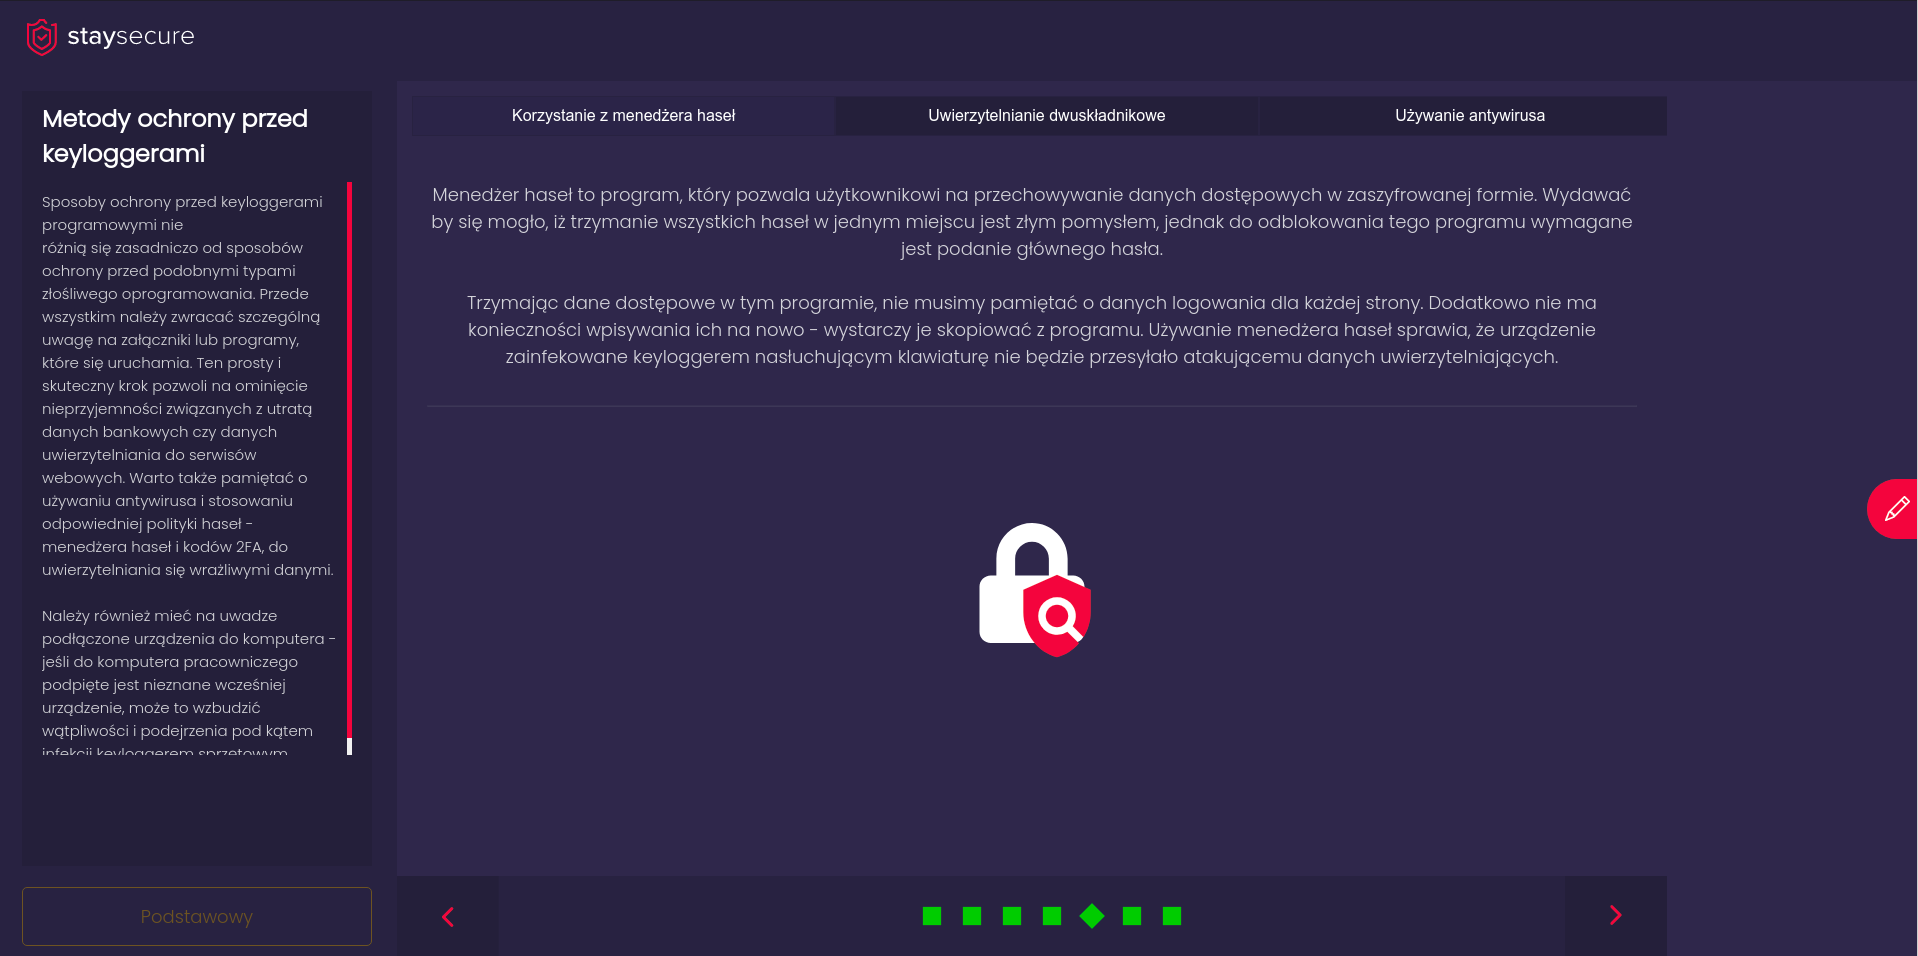
\includegraphics[width=1\linewidth]{figures/keylogger-slide-screenshot2}
	\caption{Slajd przedstawiający metody ochrony przeciw keyloggerami. Źródło: opracowanie własne}
\end{figure}

Kurs prezentuje scenariusz urządzenia zainfekowanego keyloggerem programowym oraz opisuje podstawowe elementy składające się na to zagrożenie. Poprzez udział w tym kursie, użytkownicy mają szansę zaznajomić się z mechanizmami działania keyloggerów oraz ich typami, dzięki czemu istnieje szansa, że będą zwracali większą uwagę na podejrzane procesy działające w tle, czy nieznane urządzenia podłączone do ich komputera w biurze.

\begin{comment}
//v1 
Głównym celem tego oprogramowania jest zbieranie danych o tym, jakie klawisze na klawiaturze zostały naciśnięte przez użytkownika w jakiej kolejności, a następnie okresowe wysyłanie zebranych informacji do atakującego. Posiadając wiedzę na temat tego, co zostało wpisane na urządzeniu, można bez problemu uzyskać dostęp do wrażliwych informacji takich jak prywatna korespondencja, poufne dane czy hasła. Do bardziej zaawansowanych funkcji należy między innymi przesyłanie zrzutów ekranu, rejestrowanie historii otwieranych programów i przekazywanie tych informacji dalej.

Keyloggery oprócz formy programowej istnieją również jako osobne urządzenia, które podłączane są do jednostki zazwyczaj poprzez interfejs USB. Mogą także występować jako urządzenie pośredniczące pomiędzy klawiaturą a złączem USB komputera. 

Sposobem na unikanie tego typu oprogramowania jest przede wszystkim systematyczne sprawdzanie uruchomionych procesów, ale także używanie odpowiedniego antywirusa.
\end{comment}
\clearpage

\begin{comment}
not finished
\subsection{CSRF}
Cross Site Request Forgery (CSRF) jest atakiem na aplikacje internetowe, którego celem jest wykonanie przez użytkownika końcowego niechcianej akcji w serwisie w którym aktualnie jest on zalogowany. 
[FORMAT ROZBIC WYZEJ NA DWA]


Ten typ ataku jest wykorzystywany szczególnie gdy oprogramowanie serwisu internetowego nie jest wykonane zgodnie ze standardami bezpieczeństwa OWASP (ang. Open Web Application Security Project). \cite{OWASP10}.

Warunkiem koniecznym na wystąpienie tej podatności jest aktywna sesja użytkownika w danej witrynie webowej oraz aktywny token autoryzacyjny (uzyskiwany zazwyczaj jako odpowiedź serwera na poprawne dane użytkownika przy mechanizmie logowania na stronie internetowej). Następnie przechowywany jest on w pamięci przeglądarki przez wybrany okres czasu.

Spreparowane żądanie może być stworzone na wiele sposobów. Dla przykładu, w sytuacji w której klient banku chce wykonać przelew bankowy, utworzone żądanie w podatnej, błędnie wykonanej aplikacji będzie miało następującą formę:

\

\begin{lstlisting}[caption=Przykładowe żądanie aplikacji podatnej na CSRF,label={KodPHP1}]
	GET https://bank.com/transfer?amount=100&accountNumber=123456 HTTP/1.1. 
\end{lstlisting}

Jeśli dojdzie do sytuacji że w przeglądarce będzie znajdywał się token autoryzacyjny zapisany w ciasteczkach lub pamięci lokalnej, ofiara po wejściu  w hiperłącze \
{https://bank.com/transfer?amount=100\&accountNumber=123} nieświadomie wykona to żądanie, co będzie skutkowało przelaniem określonej kwoty pieniędzy na wybrane konto przez atakującego. Link ten może zostać dostarczony poprzez stosowanie odpowiednich środków psychologicznych i metod manipulacji (inżynierię społeczną) lub maile phishingowe. Aplikacja nie jest w stanie odróżnić czy żądanie od klienta końcowego przyszło zgodne z jego intencjami, czy też nie. 

W dzisiejszych czasach, zdecydowana większość szkieletów do tworzenia aplikacji webowych posiada mechanizmy zabezpieczające budowaną stronę przed tą podatnością. Jeśli jednak wybrana technologia nie posiada wbudowanego mechanizmu, koniecznym będzie dodanie tokenów CSRF do wszystkich żądań wpływających na stan aplikacji. Z każdym żądaniem do serwera powinien być wysyłany jednorazowy token - ciąg losowych znaków, a następnie powinien być on walidowany wraz z wszystkimi danymi które znajdują się w ciele lub parametrach żądania. 


\clearpage
\end{comment}

\section{Podsumowanie i wnioski końcowe}

W czasach powszechnej komunikacji zdalnej wiedza na temat zagrożeń w sieci jest bardzo poszukiwana i cenna. Tematyka cyberbezpieczeństwa przechodzi do codzienności, czego dowodem mogą być liczne szkolenia organizowane przez firmy lub komiksy dla dzieci, przedstawiające podstawy tego obszernego zagadnienia \cite{Edukomiks}.

%Stworzony materiał szkoleniowy ma potencjał do bycia wykorzystanym do celów komercyjnych, przykładowo w małych i średnich przedsiębiorstwach, do edukacji pracowników zmieniających tryb pracy na zdalny. Istnieje również szansa na utworzenie kursów premium dla zwykłych użytkowników, które dostępne byłyby tylko dla kursantów, którzy zechcą wesprzeć projekt finansowo. Wiedza dostarczana w kursach jest uniwersalna, gdyż podstawowe koncepty zagrożeń oraz metody ochrony przed nimi rzadko są zmienne. W kursach zostały wykorzystane elementy usprawniające naukę, takie jak wykorzystanie wirtualnej rzeczywistości w stopniu podstawowym, interaktywne slajdy, notatnik pozwalający na zapisywanie cennych informacji czy quiz podsumowujący dany kurs i przedstawiający wynik kursanta. Dodatkowo, wykorzystanie narzędzia pozwalającego na przetłumaczenie aplikacji oraz treści kursów, pozwala rozszerzyć grupę docelową na nowe, zagraniczne rynki.

Stworzony materiał szkoleniowy ma potencjał do bycia wykorzystanym do celów komercyjnych, przykładowo w małych i średnich przedsiębiorstwach, do edukacji pracowników zmieniających tryb pracy na zdalny. W aplikacji zaimplementowana została funkcjonalność pobierania zawartości kursów w formacie \emph{pdf}, jednak jest ona dostępna tylko dla kursantów, którzy zechcą wesprzeć projekt finansowo. W przyszłości mogą zostać również dodanie kursy z dostępem wyłącznie dla użytkowników o typie konta premium. 

Wiedza dostarczana w kursach jest uniwersalna, gdyż podstawowe koncepty zagrożeń oraz metody ochrony przed nimi rzadko są zmienne. W kursach zostały wykorzystane elementy usprawniające naukę, takie jak wykorzystanie wirtualnej rzeczywistości w stopniu podstawowym, interaktywne slajdy, notatnik pozwalający na zapisywanie cennych informacji czy quiz podsumowujący dany kurs i przedstawiający wynik kursanta. Dodatkowo, wykorzystanie narzędzia pozwalającego na przetłumaczenie aplikacji oraz treści kursów, pozwala rozszerzyć grupę docelową na nowe, zagraniczne rynki.

Doświadczenie pisania manuskryptu pracy inżynierskiej, jak i tworzenia aplikacji internetowej przyniosło wiele korzyści: nie tylko pogłębiona została wiedza z zakresu programowania aplikacji webowych i tych działających po stronie serwera, ale również wymagane było zapoznanie się z szeroko pojętym zakresem cyberbezpieczeństwa. Poprzez staranne opisanie i zaprezentowanie różnych zagadnień niebezpieczeństw w sieci, wiedza zdobyta podczas studiów, jak i zgłębiania się w literaturę została odpowiednio usystematyzowana. Do wyników pracy zaliczyć można:
\begin{itemize}

\item naukę technologii programistycznych w celu stworzenia strony internetowej i aplikacji działającej po stronie serwera,
\item zapoznanie się z literaturą i systematyką zagrożeń w sieci oraz atakami na systemy teleinformatyczne,
\item szczegółowy opis wybranych niebezpieczeństw,
\item utworzenie systemu klasy e-learning,
\item przygotowanie treści szkoleniowych z elementami interakcji i wirtualnej rzeczywistości.
\end{itemize}
Jeśli ktoś nadal uważa, że kwestie związane z zagrożeniami w sieci są marginalne, lub obecnie stanowią jedynie mniej istotną część szeroko rozumianej teleinformatyki, a skutki nie mają tak znaczącego wpływu na indywidualne osoby, powinien zwrócić uwagę na niedawną lukę typu 0-day w postaci błędu w oprogramowaniu Log4j, która dotyczyła tysięcy przedsiębiorstw na całym świecie i wywołała panikę w branży technologii teleinformatycznych \cite{Log4j}.

\clearpage

\addcontentsline{toc}{section}{Literatura}

\begin{thebibliography}{4}
\bibitem{VrLearning}
Virtual Reality in the Learning Process, Bayron Chavez, Sussy Bayona
\bibitem{JavascriptPopularity} Amantia Pano Daniel Graziotin Pekka Abrahamsson, Factors and actors leading to the adoption of a JavaScript framework 
\bibitem{JS} https://developer.mozilla.org/en-US/docs/Learn/JavaScript/First{\_}steps/What{\_}is{\_}JavaScript. Dostęp 11.06.2021.
\bibitem{ReactPopular} Most popular web frameworks among developers worldwide 2021, Shanhong Liu, 15.12.2021
\bibitem{NodejsWhatIs} Using Node.Js to Build High Speed and Scalable Backend Database Server, S. L. Bangare, S. Gupta, M. Dalal, A. Inamdar
\bibitem{BigData} Raport ITwiz: Internet Rzeczy i Big Data w praktyce
\bibitem{Deepl}
https://www.deepl.com/en/blog/how-does-deepl-work. Dostęp 30.01.2022
\bibitem{PhishingChart} https://securelist.com/spam-and-phishing-in-q1-2021/102018. Dostęp 02.09.2021.
\bibitem{PhishingRanking} https://securelist.com/spam-and-phishing-in-q2-2021/103548. Dostęp 14.09.2021
\bibitem{PhishingEmails} Phishing Attacks: A Recent Comprehensive Study and a New Anatomy, Chaminda Hewage, Liqaa Nawaf, Imtiaz Ali Khan, Zainab Alkhalil
\bibitem{PhishingExample} https://www.egospodarka.pl/art/galeria/39266,Bankowosc-online-a-zabezpieczenia,1,12,1.html. Dostęp 01.10.2021.
\bibitem{WebScrapping} https://www.imperva.com/learn/application-security/web-scraping-attack. Dostęp 29.09.2021.
\bibitem{WhatIsPhishing} Tom N Jagatic, Nathaniel A Johnson, Markus Jakobsson, Filippo Menczer, Social phishing (2007/10/1)
\bibitem{XSSReport} https://www.wordfence.com/learn/how-to-prevent-cross-site-scripting-attacks. Dostęp 28.09.2021.
\bibitem{SameOriginPolicy} https://developer.mozilla.org/en-US/docs/Web/Security/Same-origin{\_}policy. Dostęp 12.06.2021.
\bibitem{DOM} https://developer.mozilla.org/en-US/docs/Web/API/Document{\_}Object{\_}Model. Dostęp 12.06.2021. 
\bibitem{Cookies} https://developer.mozilla.org/en-US/docs/Web/HTTP/Cookies. Dostęp 12.06.2021.
\bibitem{XSSProtection} Prevention Of Cross-Site Scripting Attacks (XSS) On Web Applications In The Client Side, S.Shalini, S.Usha
\bibitem{XSSSpecialTags} https://dev.w3.org/html5/html-author/charref. Dostęp 28.09.2021.
\bibitem{RansomwareTime} https://thedfirreport.com/2020/10/18/ryuk-in-5-hours. Dostęp 03.08.2021.
\bibitem{RansomwareAttackVectors} https://www.coveware.com/blog/ransomware-attack-vectors-shift-as-new-software-vulnerability-exploits-abound. Dostęp 02.08.2021.
\bibitem{RDP} https://docs.microsoft.com/en-us/troubleshoot/windows-server/remote/understanding-remote-desktop-protocol. Dostęp 02.08.2021.
\bibitem{Ddos} https://www.cloudflare.com/learning/ddos/what-is-a-ddos-attack. Dostęp 24.06.2021.
\bibitem{3WayHandshake} https://www.sciencedirect.com/topics/computer-science/three-way-handshake. Dostęp 19.09.2021.
\bibitem{ThreeWayHandshakePicture} https://www.luxoft-training.com/news/building-java-client-server-applications-with-tcp. Dostęp 06.02.2022
\bibitem{DDosHowItWorks} DoS and DDoS Attacks: Impact, Analysis and Countermeasures, Nikhil Tripathi, Babu Mehtre
\bibitem{DDosDetection} A novel approach for mitigating the effects of the TCP SYN flood DDoS attacks, Mitko Bogdanowski, Aleksandar Toshevski, Marjan Bogdanoski, Dimitar Bogatinov
\bibitem{Log4j} https://nvd.nist.gov/vuln/detail/CVE-2021-44228, Dostęp 04.02.2022
\bibitem{Edukomiks} https://edukomiks.pl, Dostęp 04.02.2022

\bibitem{sekurak} M. Bentkowski, G. Coldwind , A. Czyż, R. Janicki, J. Kamiński, A. Michalczyk, M. Niezabitowski, M. Piosek, M. Sajdak, G. Trawiński, B. Widła. Bezpieczeństwo aplikacji webowych
\bibitem{OWASP10} https://owasp.org/www-project-top-ten. Dostęp 10.07.2021.

\end{thebibliography}

\clearpage

\makesummary

\end{document} 
